\documentclass[12pt,a4paper,notitlepage,twoside]{book}


\usepackage{graphicx}
\usepackage[utf8]{inputenc}
\usepackage[portuguese,english]{babel}
%\usepackage[portuguese]{babel}
\usepackage[T1]{fontenc}
\usepackage{amsmath,amssymb}
\usepackage{amsthm,amsfonts}
\usepackage{color}
\usepackage[colorlinks]{hyperref}
\usepackage{abntex2abrev}
\usepackage{setspace}
\usepackage[toc,page]{appendix}

\usepackage{listings}         % Code blocks
\usepackage{cite}             % BibTeX citations
\usepackage[capitalise,noabbrev]{cleveref} % Smart referencing
\usepackage{algorithm}        % Pseudocode environment
\usepackage{algpseudocode}    % Pseudocode commands
\usepackage{xcolor}           % Custom colors for code highlighting
\usepackage{xurl}             % Clickable URLs
\usepackage{multirow}         % Multirow cells
\usepackage{adjustbox}        % Resize
\usepackage{makecell}         % Allow line breaks in table cells
\usepackage{booktabs}         % Provides \toprule, \midrule, \bottomrule
\usepackage{caption}          % Consistent caption spacing and placement

\usepackage{enumerate}
\usepackage{xspace}
\usepackage{seqsplit}

\usepackage{labeltext}

\usepackage[a4paper,top=30mm,bottom=30mm,inner=30mm,outer=25mm,headheight=7mm,headsep=6mm,footskip=7mm]{geometry}

\newcommand{\modelname}[1]{\textbf{#1}\xspace}
\newcommand{\datasetname}[1]{\textbf{#1}\xspace}
\newcommand{\variant}[1]{\textit{#1}\xspace}
\newcommand{\codename}[1]{\texttt{\protect\seqsplit{#1}}}
\newcommand{\MicroTEDAClus}{\modelname{MicroTEDAClus}}
\newcommand{\MicroTEDAClusPlus}{\modelname{MicroTEDAClus+}}
\newcommand{\StreamKM}{\modelname{StreamKM}}
\newcommand{\DenStream}{\modelname{DenStream}}
\newcommand{\CluStream}{\modelname{CluStream}}
\newcommand{\CEDAS}{\modelname{CEDAS}}
\newcommand{\TEDACloud}{\modelname{TEDACloud}}
\newcommand{\AutoCloud}{\modelname{AutoCloud}}
\newcommand{\Cassini}{\datasetname{Cassini}}
\newcommand{\BenchmarkOne}{\datasetname{StreamBenchmark(1)}}
\newcommand{\BenchmarkTwo}{\datasetname{StreamBenchmark(2)}}
\newcommand{\RandomRBFGeneratorEvents}{\datasetname{RandomRBFGeneratorEvents}}
\newcommand{\ChameleonDSThree}{\datasetname{DS3}}
\newcommand{\ChameleonDSFour}{\datasetname{DS4}}
\newcommand{\DBSTREAM}{\modelname{DBSTREAM}}
\newcommand{\BIRCH}{\modelname{BIRCH}}
\newcommand{\MiniBatchKMeans}{\modelname{Mini-batch k-means}}
\newcommand{\BICO}{\modelname{BICO}}
\newcommand{\InsectsAbrupt}{\datasetname{INSECTS abrupt}}
\newcommand{\InsectsIncremental}{\datasetname{INSECTS incremental}}
\newcommand{\InsectsReoccurring}{\datasetname{INSECTS incremental-reoccurring}}
\newcommand{\GasDrift}{\datasetname{Gas Sensor Array Drift}}
\newcommand{\KDDCup}{\datasetname{KDD Cup 1999}}
\newcommand{\Covertype}{\datasetname{Forest Covertype}}
\newcommand{\Pendigits}{\datasetname{Pendigits}}
\newcommand{\Shuttle}{\datasetname{Shuttle}}


\captionsetup[table]{position=top}
\captionsetup[figure]{position=bottom}
\captionsetup[algorithm]{position=top}
\captionsetup[lstlisting]{position=bottom}

\lstset{%
  basicstyle=\ttfamily\small,
  columns=fullflexible,
  breaklines=true,
  breakatwhitespace=true,
  frame=single,
  captionpos=b,
  numbers=left,
  numberstyle=\tiny,
  keepspaces=true,
  tabsize=4,
  keywordstyle=\color{blue},
  commentstyle=\color{gray},
  stringstyle=\color{green!50!black},
}

\makeindex

\linespread{1.25} %corresponde ao espaçamento 1.5 do MS Word

%---------------Início do documento-------------------------

\begin{document}

\begin{titlepage}
\begin{center}
{\large Federal University of Minas Gerais\\
School of Engineering \\
Bachelor's Degree in Control and Automation Engineering\\}

\vspace{6cm}
{\bf\Large Reassessment of the MicroTEDAClus Clustering Algorithm and Proposal for an Improved Model}
\vspace{4cm}

%\hspace{0.3\textwidth} \parbox{0.65\textwidth}
{\large Eduardo Henrique Basilio de Carvalho}
\vspace{2cm}

\vspace{2cm}
%\hspace{0.3\textwidth}
{\large Advisor: Prof. Janier Arias Garcia, PhD}

\vfill
%\hspace{0.3\textwidth}
{\large Belo Horizonte, \today }
\end{center}

\end{titlepage}

\newpage
\clearpage
\thispagestyle{empty}


\begin{titlepage}

\centering
\textbf{Undergraduate Thesis}\\
\vspace{2cm}
\centering
\textbf{Reassessment of the microTEDAclus Clustering Algorithm and Proposal for an Improved Model}\\
\vspace{5cm}

\parbox{1.0\textwidth}
{\large
Undergraduate Thesis submitted to the examination committee
designated by the Academic Board of the Bachelor's Degree in
Control and Automation Engineering at the Federal University of
Minas Gerais, as part of the requirements for approval in the
activity Projeto Final de Curso II.}

\vspace{7cm}
\centering
Belo Horizonte, \today

\end{titlepage}


\pagenumbering{roman}
\addcontentsline{toc}{chapter}{Resumo}

\begin{center}
\huge{{\bf Resumo}}
\vspace{1cm}
\end{center}

\begin{otherlanguage}{portuguese}
MicroTEDAClus é um algoritmo de agrupamento evolutivo para fluxos de dados que resume o fluxo em microgrupos por meio da excentricidade e da tipicidade do arcabouço TEDA, e cujos autores relatam ter desempenho equivalente ao de algoritmos consolidados de agrupamento de fluxos e se adaptar melhor do que eles a mudanças nos dados. Este projeto final de curso, desenvolvido na Universidade Federal de Minas Gerais, no curso de Engenharia de Controle e Automação, sob orientação do Prof. Janier Arias Garcia, reavalia o algoritmo e propõe um modelo aprimorado. A reavaliação identifica problemas na formulação do algoritmo, diferenças entre a formulação e a implementação pública que produziu os seus resultados publicados e falhas na metodologia dos seus experimentos, entre elas etapas de pré-processamento que vazam informação sobre os dados e uma avaliação que prediz cada lote depois de aprendê-lo. Sob uma metodologia sem essas falhas, na qual todos os modelos são executados na mesma linguagem sobre os dados sem pré-processamento, avaliados de forma prequencial, ajustados pela mesma busca de hiperparâmetros e comparados por testes estatísticos em muitas execuções, o MicroTEDAClus não tem desempenho equivalente ao dos modelos de referência do trabalho original, nem se adapta melhor do que eles a mudanças de conceito.

O modelo aprimorado, MicroTEDAClus+, resulta de experimentos controlados nos quais cada correção ou modificação é aceita por uma regra definida previamente, em execuções separadas das da sua avaliação. Nos conjuntos de dados sintéticos do trabalho original, ele supera o MicroTEDAClus em qualidade de agrupamento, tempo de execução e memória, nenhum modelo de referência o supera nos conjuntos com mudança de conceito, e ele é o mais rápido desse experimento. Em um experimento modernizado no ambiente, nos modelos de referência e na seleção de hiperparâmetros, ele supera todos os modelos de referência em alguns conjuntos de dados e é superado por todos em outros. Em oito conjuntos de dados reais, porém, ele é superado pela maioria dos modelos de referência em seis. Um diagnóstico e novos experimentos controlados nesses conjuntos produzem a versão final do MicroTEDAClus+, que reduz a faixa de busca do seu limite de variância, abandona o rótulo de ruído e busca o fator que liga os seus microgrupos. Ela é superada pela maioria dos modelos de referência em três conjuntos de dados reais, em vez de seis, e supera todos em um, mas segue atrás de alguns nos fluxos reais com mudança de conceito.

\noindent\textbf{Palavras-chave:} Agrupamento de fluxos de dados. Agrupamento evolutivo. TEDA. Mudança de conceito. Metodologia experimental.
\end{otherlanguage}

\clearpage
\thispagestyle{empty}
\cleardoublepage

\addcontentsline{toc}{chapter}{Abstract}

\begin{center}
\huge{{\bf Abstract}}
\vspace{2cm}
\end{center}

MicroTEDAClus is an evolving clustering algorithm for data streams that summarizes the stream into microclusters by the eccentricity and the typicality of the TEDA framework, and whose authors report that it performs on par with established stream clustering algorithms and adapts better than them to changes in the data. This undergraduate thesis, developed at the Federal University of Minas Gerais in the Bachelor's Degree in Control and Automation Engineering, under the supervision of Prof. Janier Arias Garcia, reassesses the algorithm and proposes an improved model. The reassessment finds issues in the formulation of the algorithm, differences between the formulation and the public implementation that produced its published results, and flaws in the methodology of its experiments, among them preprocessing steps that leak information about the data and an evaluation that predicts each batch of samples after learning it. Under a methodology without these flaws, in which every model is executed in the same language on the unprocessed data, evaluated prequentially, tuned by the same automatic search and compared over many runs by nonparametric statistical tests, MicroTEDAClus is frequently outperformed by the benchmark models, and its claimed adaptability is not supported in full.

The improved model, MicroTEDAClus+, results from controlled experiments in which each correction or modification is accepted by a predefined rule, on runs separate from those of its evaluation. On the synthetic datasets of the original work it improves on MicroTEDAClus in clustering quality, execution time and memory, it is among the best benchmark models in the datasets with concept drift and the fastest of them, and in an experiment modernized in its environment, its benchmark models and its selection of hyperparameters it remains among the best models in most datasets. On eight real datasets, however, it is among the worst models. A diagnosis and a second effort of controlled experiments on those datasets produce the final version of MicroTEDAClus+, which lowers the search range of its variance limit, drops its noise label and searches the factor that links its microclusters. It is no longer among the worst models in most real datasets and is the best in one of them, but it remains behind the best benchmark models on the real streams with concept drift.

\clearpage
\thispagestyle{empty}
\cleardoublepage

\addcontentsline{toc}{chapter}{Acknowledgements}

\begin{center}
\huge{{\bf Acknowledgements}}
\vspace{4cm}
\end{center}

Write the acknowledgements here. You can thank your advisors, colleagues, friends, and family for their support and contributions to your work.

\clearpage
\thispagestyle{empty}
\cleardoublepage

\tableofcontents
%\markboth{Conteúdo}{Conteúdo}

\clearpage
%\thispagestyle{empty}
%\cleardoublepage

% Normalmente, este arquivo só contém isto.

\listoffigures
\addcontentsline{toc}{chapter}{Figures List}
%\markboth{Lista de Figuras}{Lista de Figuras}

\clearpage
%\thispagestyle{empty}
%\cleardoublepage

% Normalmente, este arquivo só contém isto.

\cleardoublepage
\phantomsection
\addcontentsline{toc}{chapter}{\listtablename}
\listoftables
%\markboth{Lista de Tabelas}{Lista de Tabelas}

\clearpage
%\thispagestyle{empty}
%\cleardoublepage

% Normalmente, este arquivo só contém isto.


\pagenumbering{arabic}
\setcounter{page}{1}
\chapter{Introduction}
\label{chap:intro}

Data streams arrive continuously and without a known end, and the process that generates them can change while they are observed. Clustering such a stream requires an algorithm that processes each sample as it arrives, keeps a bounded summary of what it has seen and follows the changes of the data, a family of methods known as stream or evolving clustering \cite{aggarwal2003framework,cao2006density,wang2023data}. \MicroTEDAClus \cite{maia2020evolvclus} is one such algorithm. It summarizes the stream into microclusters by the eccentricity and the typicality of the TEDA framework \cite{angelov2014outside}, which assume no distribution for the data and are computed recursively, and it groups the microclusters into macroclusters that represent the clusters of the stream. Its authors report that it performs on par with established stream clustering algorithms, and that it adapts better than them to concept drift.

This work reassesses \MicroTEDAClus and proposes an improved model. The reassessment finds issues in the formulation of the algorithm, differences between the formulation and the implementation that produced the published results, and flaws in the methodology of the original experiments, among them preprocessing steps that leak information about the stream and an evaluation that predicts each batch after learning it. Under a methodology that corrects these flaws, \MicroTEDAClus is frequently outperformed by the benchmark models. The improved model, \MicroTEDAClusPlus, is the result of controlled experiments on corrections and modifications of the algorithm. On the synthetic datasets of the original work it improves on \MicroTEDAClus in clustering quality, execution time and memory, and it is among the best benchmark models in the datasets with concept drift. In an experiment modernized in its environment, its benchmark models and its selection of hyperparameters, it remains indistinguishable from the best model in most datasets. On real datasets, however, it is among the worst models. A second effort of controlled experiments on those datasets produces the final version of \MicroTEDAClusPlus, which is no longer among the worst models in most real datasets and is the best in one of them, while it remains behind the best models on the real streams with concept drift.

\section{Motivation}
\label{sec:motivation}

The results of \MicroTEDAClus are the basis of later work. The doctoral thesis of \cite{galindo2021lastmile} updates the algorithm and applies it to the last-mile problem in logistics, assuming the validity of the original evaluation without examining it. A model whose evaluation supports further work must be verified, and the verification of empirical results in machine learning is not a formality: information leaked from the data into the evaluation, among other errors, has been found to inflate the published results of many studies \cite{kaufman2012leakage,kapoor2023leakage}. The algorithm is also attractive for what it promises. The TEDA metrics require neither a distribution for the data nor a predefined number of clusters, and an algorithm built on them that is accurate, fast and robust to concept drift would be a useful tool for stream clustering.

The datasets of the original work are synthetic streams and benchmarks of static shapes, whose clusters, drifts and noise are known by construction. A model that is to serve applications must also be judged on data recorded from physical processes, whose classes are not drawn from chosen distributions and whose drifts come from the conditions of the recording. An evaluation on real data tests whether the conclusions reached on synthetic data hold.

This work verifies the claims of \MicroTEDAClus before building on them, and improves the model where the verification shows weaknesses. The TEDA framework is that of \cite{angelov2014outside}. The formulation of \MicroTEDAClus and its reference implementation are those of \cite{maia2020evolvclus}, and its updated formulation is that of \cite{galindo2021lastmile}. The benchmark models are those of their respective authors. In the main experiment they are executed through the implementations of the \codename{River} library \cite{montiel2021river} or, for \CEDAS, \TEDACloud and \AutoCloud, through implementations made for this work from the official code or from the descriptions in their papers; in the modernized and real-data experiments, through \codename{River}, \codename{scikit-learn} \cite{pedregosa2011scikit} and the \codename{bico} package \cite{fichtenberger2013bico}. The real datasets are those of the sources cited where they are introduced. The reassessment of the formulation, of the implementation and of the methodology, the methodology that replaces the original one, the vectorized implementation, the experiments of the improvement and \MicroTEDAClusPlus, the modernized experiment with its ported stream generators and its search ranges by rule, the real-data experiment, and the second effort of improvement with the final version of \MicroTEDAClusPlus are the contribution of this work.

\section{Objectives}
\label{sec:objectives}

From the motivation presented in the previous section, the objectives of this work are:

\begin{enumerate}[a)]
\item to examine the formulation of \MicroTEDAClus and its public implementation, and identify their issues and the differences between them;
\item to examine the methodology of the experiments of the original work, and define a methodology that evaluates every model alike and without its flaws;
\item to evaluate \MicroTEDAClus against benchmark models under that methodology;
\item to propose an improved model by controlled experiments on the issues identified, and evaluate it under the same methodology against \MicroTEDAClus and the benchmark models;
\item to modernize the experiment, with a single environment, benchmark models from maintained libraries, a selection of hyperparameters that depends neither on the scale of the data nor on the speed of the machine, and the cost of every model measured with each task executed alone, and to evaluate the improved model under it;
\item to evaluate the improved model on real datasets and, where it falls short, improve it again by controlled experiments, and compare the result with the benchmark models.
\end{enumerate}

\section{Structure of the Thesis}
\label{sec:structure}

The work is divided into nine chapters besides this introduction. \Cref{chap:background_relatedwork} presents the TEDA framework, the formulation of \MicroTEDAClus and its update, together with the issues of both. \Cref{chap:methodology_reassessment} examines the implementation of \MicroTEDAClus and the methodology of the original experiments, defines the methodology of this work and evaluates \MicroTEDAClus and the benchmark models under it. \Cref{chap:ModelImprovement} optimizes the implementation, evaluates corrections and improvements of the algorithm, defines \MicroTEDAClusPlus and compares it with \MicroTEDAClus in the main experiment. \Cref{chap:results} places \MicroTEDAClusPlus among the benchmark models. \Cref{chap:modernization} replaces the environment, the benchmark models and the selection of hyperparameters, and repeats the main experiment under them. \Cref{chap:real_data} evaluates the models on real datasets. \Cref{chap:real_improvement} diagnoses \MicroTEDAClusPlus on those datasets, improves it again and compares its final version with the benchmark models. \Cref{chap:discussion} reads the results of these chapters together, and \cref{chap:conclusions} summarizes the findings, their limits and the directions of future work. \Cref{app:mi_tables} collects complementary tables of the experiments of \cref{chap:ModelImprovement}.

\clearpage

\chapter{Background and Related Work}
\label{chap:background_relatedwork}

This chapter presents the eccentricity and the typicality of the TEDA framework (\cref{sec:teda}), the formulation of \MicroTEDAClus by Maia et al.\ (\cref{sec:original_formulation}), its update by Galindo (\cref{sec:updated_formulation}), and the reimplementation of the model in \codename{C} by Cardoso (\cref{sec:c_implementation}). After each formulation, we discuss its issues, and we point to where the following chapters examine them.

\section{Typicality and Eccentricity-Based Data Analytics}
\label{sec:teda}

Angelov~\cite{angelov2014outside} introduces the TEDA framework as an alternative to probability theory for data in non-deterministic settings, built on two metrics. The eccentricity $\xi^k_j$ of a sample $j$ at moment $k$, twice the sum $\pi^k_j$ of its distances to all the samples seen up to $k$ divided by the sum of these sums over all the samples, measures how much the sample deviates from the others, and its typicality $\tau^k_j = 1 - \xi^k_j$ how well it fits among them; both lie between zero and one once $k > 2$ and the sums are positive. Their normalized forms are

\begin{equation}
    \zeta^k_j = \frac{\xi^k_j}{2}, \qquad t^k_j = \frac{\tau^k_j}{k - 2}, \qquad \sum_{i=1}^{k} \zeta^k_i = \sum_{i=1}^{k} t^k_i = 1,
    \label{eq:normalized_typicality}
\end{equation}

and a sample is anomalous if $\zeta^k_j > 1/k$ and typical if $t^k_j > 1/k$. For the squared Euclidean distance, the sums of the distances can be updated recursively from the mean and the mean squared norm of the samples.

Angelov also states that \labeltext[Angelov's statement about the use of other proximity functions]{the metrics suit other proximity functions, among them the cosine similarity and the Mahalanobis distance}{info:mahalanobis_as_teda_metric}~\cite{mahalanobis1936generalized}.

\section{Original MicroTEDAClus}
\label{sec:original_formulation}

Maia et al.~\cite{maia2020evolvclus} use the eccentricity and the typicality over the Euclidean distance to create and update microclusters, by detecting outliers and typical samples, and to merge the microclusters into macroclusters. They write the eccentricity in the recursive form

\begin{equation}
    \xi(x_k) = \frac{1}{k} + \frac{\left( \mu_k - x_k \right)^T \left( \mu_k - x_k \right)}{k \sigma^2_k}, \label{eq:recursive_eccentricity}
\end{equation}

with

\begin{gather}
    \mu_k = \frac{k - 1}{k} \mu_{k-1} + \frac{x_k}{k}, \qquad
    \sigma^2_k = \frac{k - 1}{k} \sigma^2_{k-1} + \frac{1}{k - 1} \lVert x_k - \mu_k \rVert^2,
\end{gather}

and consider a sample an outlier if $\zeta(x_k) > (m^2 + 1)/(2k)$, with $m > 0$ a function of the number of samples chosen by the authors,

\begin{equation}
    m(k) = \frac{3}{1 + e^{-0.007(k - 100)}}.
    \label{eq:m_function}
\end{equation}

A microcluster $i$ at moment $k$ is described by its number of samples $S^i_k$, the mean $\mu^i_k$ and the variance $(\sigma^i_k)^2$ of its samples, the eccentricity $\xi^i(x_k)$, the typicality $\tau^i(x_k)$ and their normalized forms $\zeta^i(x_k)$ and $t^i(x_k)$ of a sample $x_k$ to it, \labeltext[order-dependent parameter handled as a characteristic of the microcluster]{its density $D^i_k = 1 / \zeta^i(x_k)$}{critique:density_as_microcluster_characteristic}, and its threshold function $m^i_k(S^i_k)$. The metrics apply to each microcluster as to the whole data. For $S^i_k > 2$, a sample $x_k$ is an outlier to microcluster $i$ if

\begin{equation}
    \zeta^i(x_k) > \frac{m^i_k(S^i_k)^2 + 1}{2S^i_k}, \label{eq:outlier_condition}
\end{equation}

and, for $S^i_k = 2$, if

\begin{equation}
    \left( \zeta^i(x_k) > \frac{m^i_k(2)^2 + 1}{4} \right) \land \left( \left( \sigma^i_k \right)^2 < r_0 \right), \label{critique:incorrect_condition_logic}
\end{equation}

where $r_0$ is a hyperparameter, the variance limit. Every microcluster to which $x_k$ is not an outlier is updated by

\begin{equation}
\begin{gathered}
    S^i_k = S^i_{k-1} + 1, \qquad
    \mu^i_k = \frac{S^i_k - 1}{S^i_k} \mu^i_{k-1} + \frac{x_k}{S^i_k}, \\
    \left(\sigma^i_k\right)^2 = \frac{S^i_k - 1}{S^i_k} \left(\sigma^i_{k-1}\right)^2 + \frac{1}{S^i_k - 1} \left( \frac{2\lVert x_k - \mu^i_k \rVert }{d} \right)^2, \\
    \xi^i(x_k) = \frac{1}{S^i_k} + \frac{2\left( \mu^i_k - x_k \right)^T \left( \mu^i_k - x_k \right)}{S^i_k \left( \sigma^i_k \right)^2d},
\end{gathered} \label{critique:dimensionality_penalty}
\end{equation}

where $d$ is the dimension of the data. A sample that is an outlier to every microcluster creates a new one, with one sample, its mean at the sample and no variance, as the first sample of the stream does.

The macroclusters are the connected components of the graph whose vertices are the microclusters and whose edges join the microclusters that satisfy

\begin{equation}
    \text{dist}(\mu^i_k, \mu^j_k) < 2 \left( \sigma^i_k + \sigma^j_k \right), \quad i \neq j. \label{eq:microcluster_intersection_condition}
\end{equation}

\labeltext[criterion to prevent microcluster collapse]{To keep overlapping microclusters from collapsing into a single macrocluster, a microcluster $m^j_l$ takes part in the macrocluster $\mathcal{M}_j = \{ m^j_1, \dots, m^j_{N_j} \}$ only if it is active, that is, if}{info:microcluster_activation_criterion}

\begin{equation}
    D^l_k \ge \text{mean}\left(D^l_k\right), \quad l = 1,\dots,N_j. \label{critique:use_of_unstable_density}
\end{equation}

Each active microcluster weighs in its macrocluster by its share of the density of the active microclusters, and the typicality of a sample $x_k$ to a macrocluster is the weighted sum of its typicalities to them,

\begin{equation}
    \mathcal{T}_j(x_k) = \sum_{l\in\mathcal{M}_j} \frac{D^l_k}{\sum_{l'\in\mathcal{M}_j} D^{l'}_k}\, t^l_k(x_k), \label{eq:macrocluster_typicality}
\end{equation}

the sample being assigned to the macrocluster of highest typicality. The formulation defines no decay of the microclusters, although the public implementation has one (\cref{sec:model_implementation}).

\subsection{Issues of the Original Formulation}

\paragraph{Order-dependent density.}
\label{subsubsec:order_dependent_characteristics}
The eccentricity and the typicality relate a sample to a microcluster, so the density $D^i_k = 1 / \zeta^i(x_k)$ relates them too, and should not be treated as a property of the microcluster. A microcluster with a small variance is dense for any standard clustering algorithm~\cite{ester1996density,aggarwal2003framework,cao2006density}, but if the current sample is far from its mean, $\zeta^i(x_k)$ is large and $D^i_k$ small, and the microcluster is less likely to be activated. Conversely, a microcluster with a large variance and a sample close to its mean has a large $D^i_k$ and is more likely to be activated, even if it is not dense at all. \Cref{sec:mi_corrections} tests two densities that do not depend on the current sample, and \cref{subsec:mi_not_retained} tests both again on \MicroTEDAClusPlus.

\paragraph{Outlier condition for microclusters with two samples.}
\label{subsubsec:incorrect_condition_logic}
For $S^i_k = 2$, \cref{eq:recursive_eccentricity} and the recursion of the mean and the variance give

\begin{gather}
    \mu_2 = \frac{1}{2} \left( x_1 + x_2 \right), \qquad
    \sigma^2_2 = \lVert x_2 - \mu_2 \rVert^2, \qquad
    \xi(x_2) = 1, \qquad
    \zeta(x_2) = 0.5,
\end{gather}

and, because $m \ge 1$,

\begin{equation}
    \frac{m^i_k(2)^2 + 1}{4} \ge 0.5.
\end{equation}

The first term of \cref{critique:incorrect_condition_logic} is therefore never satisfied, and neither is the conjunction: no sample can be an outlier to a microcluster with two samples. With the scaled expressions of \cref{critique:dimensionality_penalty}, the normalized eccentricity of the second sample becomes $1/4 + d/8$, so the first term is never satisfied with one or two dimensions and always satisfied with three or more, where the condition reduces to $\left( \sigma^i_k \right)^2 < r_0$, which holds for the samples close to the mean. Either way, the condition does not detect outliers. Replacing it by

\begin{equation}
    \left( \sigma^i_k \right)^2 < r_0
    \label{eq:corrected_condition_logic}
\end{equation}

would keep the inversion, so the condition should be

\begin{equation}
    \left( \sigma^i_k \right)^2 > r_0.
    \label{eq:corrected_condition_logic_for_outliers}
\end{equation}

Cardoso~\cite{cardoso2022microtedaclus} reached the same conclusion earlier, proving that the eccentricity of the second sample is always one, and detects the outliers of microclusters with fewer than three samples by \cref{eq:corrected_condition_logic_for_outliers} alone, as the public implementation does (\cref{sec:model_implementation}).

\paragraph{Dimensionality penalty.}
\label{subsubsec:dimensionality_penalty}
\Cref{critique:dimensionality_penalty} scales the variance and the eccentricity of a microcluster by the dimension $d$. No paper that introduces the TEDA metrics suggests such a scaling~\cite{angelov2014outside,angelov2014anomaly}, the original work does not justify it, and it lets the normalized eccentricity exceed its bound of one half. \Cref{sec:reassessment_results} traces the collapse of \MicroTEDAClus in high dimensions to it, and \cref{sec:mi_corrections} tests its removal.

\section{Updated MicroTEDAClus}
\label{sec:updated_formulation}

In the PhD thesis \textit{Mineração de Dados Aplicada a Problemas de Last-Mile na Logística}, Galindo~\cite{galindo2021lastmile} updates \MicroTEDAClus to apply it to the last-mile problem in logistics; we describe only the changes. It introduces an explicit decay: each microcluster has a vitality $v^i_k$, set to one when it is created and lowered by

\begin{equation}
    v^i_k = v^i_{k-1} - \rho
    \label{eq:decay_logic}
\end{equation}

whenever the sample $x_k$ is an outlier to it, where $\rho = 1/\text{decay}$ and \textit{decay} is a hyperparameter, and a microcluster is removed when $v^i_k \le 0$. \Cref{sec:mi_improvements} tests this rule as the candidate \variant{recency}. The update also corrects the direction of the comparison with $r_0$ in the condition for microclusters with two samples, but keeps its conjunction, and replaces the Euclidean distance by the cosine similarity, with the outlier condition that Angelov~\cite{angelov2014anomaly} derives for the Euclidean distance and a variance that remains Euclidean, neither of them justified for the new distance. The order-dependent density and the dimensionality penalty remain, and the rest of the algorithm is unchanged.

\section{A \texttt{C} Implementation of MicroTEDAClus}
\label{sec:c_implementation}

In the undergraduate thesis \textit{Implementação do algoritmo MicroTEDAclus para classificação de dados}, Cardoso~\cite{cardoso2022microtedaclus} reimplements the original \MicroTEDAClus in \codename{C}, a language chosen for its speed and for its use in embedded platforms. The thesis documents the TEDA expressions that the model uses, with proofs and unit tests, and proposes an alternative to the intersection condition of \cref{eq:microcluster_intersection_condition}, which compares the distance between the means of two microclusters with the sum of their radii $m^i_k(S^i_k)\,\sigma^i_k$, scaled by a factor $\phi$:

\begin{equation}
    \text{dist}(\mu^i_k, \mu^j_k) < \phi \left( m^i_k(S^i_k)\,\sigma^i_k + m^j_k(S^j_k)\,\sigma^j_k \right), \quad \phi \ge 1, \quad i \neq j.
    \label{eq:cardoso_intersection_condition}
\end{equation}

Its experiments evaluate the clustering quality by the adjusted Rand index on seven static datasets of two dimensions. The model learns each whole dataset before labeling it, in random orders of the samples and with hyperparameters taken from a grid, and the thesis reports the lowest and the highest index and the highest mean index over the configurations~\cite[Section 4.3]{cardoso2022microtedaclus}. It concludes that the quality depends strongly on $r_0$ and $\phi$, and that \cref{eq:cardoso_intersection_condition} is comparable to \cref{eq:microcluster_intersection_condition}. The reimplementation runs much faster than the \codename{Python} implementation of the original work, measured over each whole program on a single machine and without repetitions~\cite[Section 4.4]{cardoso2022microtedaclus}.

\subsection{Issues of the Evaluation of the C Implementation}

The highest indices belong to the configurations of the grid that best fit the labels of the evaluated data, and are therefore optimistic estimates of the quality that the model reaches when its hyperparameters are chosen without those labels. The lowest index is no better than chance in every dataset~\cite[Tables 4.1 and 4.2]{cardoso2022microtedaclus}, and the comparison between the two intersection conditions rests on the best cases, without a statistical test. The model is compared with no benchmark model, and none of the datasets has concept drift, which the thesis expects the model to handle because the original work reports that it does~\cite[Section 4.2]{cardoso2022microtedaclus}.

\chapter{Methodology Reassessment}
\label{chap:methodology_reassessment}

The \textit{Evolving clustering algorithm based on mixture of typicalities for stream data mining} paper presents promising results for the microTEDAclus model \cite{maia2020evolvclus}. Before conclusions can be drawn from those results, however, it is important to assess the methodology used in the original work. In this chapter, only its methodology is reviewed, since the following paper, \textit{Mineração de Dados Aplicada a Problemas de Last-Mile na Logística} \cite{minerao2022minerao} assumes its validity and does not perform further investigation on it.

The next sections examine weaknesses from the evaluated model implementation to the experiments protocol, including the evaluation metrics and procedures. The goal of this reassessment is to identify potential issues in the original work's methodology that could affect the validity of its results and conclusions. By doing so, a more rigorous and accurate evaluation of the microTEDAclus model can be conducted, leading to more reliable conclusions about its performance and applicability in real-world scenarios.

\section{Model Implementation}

%% the model's implementation seen in the public repository is not the same as the one described in the original work, but much more similar to the updated version presented in the PHD thesis Mineração de Dados Aplicada a Problemas de Last-Mile na Logística. this is a problem because the results of the experiments are not comparable to the ones presented in the original work, and the conclusions drawn from those results may not be valid.

%% required bibliography:
%% - the paper that introduces the original version of microTEDAclus: Evolving clustering algorithm based on mixture of typicalities for stream data mining, by José Maia Neto
%% - the paper that introduces the updated version of microTEDAclus: Mineração de Dados Aplicada a Problemas de Last-Mile na Logística, by Juan Camilo Fonseca Galindo

In the fifth section of the original work, \textbf{Methodology and experiments}, \cite{maia2020evolvclus} provides a URL to the public GitHub repository where the code for the experiments can be found: \url{https://github.com/cseveriano/evolving_clustering}. To ensure persistence of the code, a fork of the original repository was created at the commit \texttt{50dd2b4}, which is the last commit to the repository at the time of this reassessment \cite{eduardo2026evolvingclustering}. The implementation of the microTEDAclus model is found in the \texttt{src/models/evolving/EvolvingClustering.py} file of the repository.

\section{Benchmark Models Source}

%% the models are denstream, clustream, and streamkm++ . those are suitable models for data stream clustering benchmark. the validity of the experiments, however, depends on implementation and execution

%% required bibliography:
%% - the paper that introduces DenStream:
%% - the paper that introduces CluStream:
%% - the paper that introduces StreamKM++:

\subsection{Original Work}

%% the original work states it uses R's streammoa. the problem is that, because the experiments are done in python, the package calls R, which, in turn, calls Java. this is a problem because of the overhead of calling R and Java from Python

%% required bibliography:
%% - the paper that introduces streammoa:

\subsection{Current work}

%% uses river's clustream and denstream and clusopt-core's streamkm++. river's implementations are in pure python, which make them comparable to microTEDAclus. clusopt-core's streamkm++ is implemented in C++, which makes it faster than microTEDAclus, rather than slower.

%% required bibliography:
%% - the paper that introduces river:
%% - the paper that introduces clusopt-core:

\section{Datasets}

%% although the original work references valid benchmarking datasets, the preprocessing to which those datasets are subjected before being used is omited and have a significant impact on the results.

%% required bibliography:
%% - an authority paper on the impact of preprocessing on results. not necessarily the first to talk about it, but one that is widely cited and recognized in the field:

\subsection{Static}

%% the original work uses cleaned, scaled, and downsampled versions of two of the chameleon datasets, as seem in the public repository, and the ordered, noiseless, cassini dataset from streammoa.

%% we use the same datasets, but we also include the original versions of the chameleon datasets, which are not cleaned, scaled, or downsampled. this allows us to evaluate the impact of preprocessing on the results.

%% required bibliography:
%% - the paper that introduces the chameleon datasets:
%% - link to public repository of the original work: https://github.com/eduardo-ufmg/evolving_clustering (current author's fork of the original repository at the commit 50dd2b4)

\subsection{Concept Drift}

%% the streammoa concept drift datasets used are STR-B1, STR-B2, and RBF. those are generated with noise samples labeled as 'NA'. from the scatter plots shown in the original work, it seems that the noise samples are not included in the evaluation. we will include the noise samples in the evaluation, as they are part of the dataset and can have a significant impact on the results. this allows us to evaluate the impact of noise on the results.

%% required bibliography:
%% - an authority paper on the impact of noise on results. not necessarily the first to talk about it, but one that is widely cited and recognized in the field:

\subsection{Scalability}

%% for the scalability experiments, the original work uses synthetic datasets. the generation process and conditions is well described in the original work, and lack the introduction of noise, which is a common characteristic of real-world datasets. we will generate synthetic datasets with noise, to evaluate the impact of noise on the results.

%% required bibliography:
%% - an authority paper on noise in real world datasets. not necessarily the first to talk about it, but one that is widely cited and recognized in the field:

\section{Evaluation Metrics}

%% the main quality metric used in the original work is the adjusted rand index (ARI). this is a suitable metric for clustering evaluation.
%% the statistics regarding the metric, however, is not. although the original work states that the results are averaged over multiple runs with random subsets of the data, the public repository shows that the results are obtained from a single run for each dataset. the `mean` and `std` values shown in the original work are statistics of the ARI values obtained from the different batches of data, and not from multiple runs. this is a problem because it does not reflect the true variability of the results.
%% furthermore, mean and standard deviation are only valid statistics when the results are expected to be normally distributed, which is not the case for quality metrics over sequential batches of data, where the results for each batch are not independent and are a direct consequence of the data snapshot, which is not random, since it is a sequential batch of data.

%% required bibliography:
%% - the paper that introduces the ARI metric:
%% - an authoritative paper that states that the mean and the standard deviation are suitable statistics for normally distributed data, and that they are not suitable for non-normally distributed data. not necessarily the first to talk about it, but one that is widely cited and recognized in the field:
%% - the paper that introduces the iqr metric:

\section{Prequential Versus Sequential Evaluation}

%% as can be seem in the public repository, what the paper calls "prequential evaluation" is actually a batched sequential evaluation, where the model is trained then evaluated on the same batch of data. this is a problem because it does not reflect the true performance of the model in a streaming setting, where the model is evaluated on unseen data after being trained on previous data.

%% furthermore, batched evalutation is performed solely on the concept drift datasets. static datasets are evalutated in a single fit then predict pass, which, besides not being a streaming setting, is not standard practice even for static datasets, where cross-validation is preferred. this is a problem because it does not allow us to evaluate the performance of the model on unseen data, and it does not allow us to compare the results with other works that use cross-validation.

%% code source:
%% - src/models/evolving/util/Benchmarks.py
%% - notebooks/**

%% required bibliography:
%% - an authoritative paper that explains and comments on prequential evaluation. not necessarily the first to talk about it, but one that is widely cited and recognized in the field:
%% - an authoritative paper that explains and comments on cross-validation. not necessarily the first to talk about it, but one that is widely cited and recognized in the field:

\chapter{Model Improvement}
\label{chap:ModelImprovement}

\chapter{Experiment Modernization}
\label{chap:modernization}

The main experiment of the previous chapters runs part of its models and generators in \codename{R} and \codename{Java}, as \cref{chap:methodology_reassessment} describes, and its protocol carries the constraints of that environment. Its hyperparameter search penalizes the execution time and stops at a time limit, and its datasets have at most 10000 samples, because some of the models are too slow for an unrestricted search, \cref{subsec:hyperparameter_tuning}. The ranges of that search were set by hand, as values that seemed reasonable after a brief survey of the literature, as most of the works it cites also set theirs. \Cref{sec:mi_selection} found that the objective of the search observes too short a segment of the stream to recognize the configurations that are best in the long run, and that the search is itself a source of variation.

This chapter replaces the environment, the benchmark models and the hyperparameter selection, and repeats the main experiment under them. The model it evaluates is \MicroTEDAClusPlus as \cref{sec:mi_final_model} defines it, without changes.

\section{Environment}
\label{sec:mod_environment}

The experiment is written in \codename{Python} only. Its numerical parts run in compiled code through the libraries that provide them, and no other runtime is involved. \MicroTEDAClusPlus keeps the implementation of \cref{sec:mi_final_model}. Every model is used through one interface: it predicts the labels of a batch, learns the batch, and reports the number of structures of its summary of the stream, which generalizes the microcluster count of \cref{sec:evaluation_metrics}. A sample that a model predicts before it has any cluster is labelled as noise.

\subsection{Stream Generators}
\label{subsec:mod_generators}

Four generators of \cref{sec:datasets} ran in \codename{R}: that of \Cassini and those of \BenchmarkOne, \BenchmarkTwo and \RandomRBFGeneratorEvents, the last from MOA \cite{bifet2010moa} through \codename{streamMOA} \cite{streamMOA2024}. They are ported to \codename{Python}, following their reference implementations step by step. The Chameleon datasets remain the files of \cref{sec:datasets}, and the scalability streams were already generated in \codename{Python}. A stream is determined by its dataset and its run, which seed its generator.

Each port is compared with the streams that \codename{R} generated for the previous experiment, 126 streams of each source per dataset. For the three generators whose samples are independent given the time, the distributions of the samples are compared by Kolmogorov-Smirnov tests on each coordinate of each cluster and by a chi-squared test on the cluster proportions, \cref{tab:mod_generators_distribution}. The structure of the four streams is compared through descriptors computed in windows of 500 samples, \cref{tab:mod_generators_descriptors,fig:mod_generators_descriptors}, and the behaviour of three models with fixed hyperparameters through their ARI, \cref{tab:mod_generators_behaviour}. Descriptors and behaviour are compared by the Mann-Whitney test, with the Holm correction and the threshold on Cliff's delta of \cref{sec:statistical_significance}. No test finds a difference in the distributions of the samples, in the descriptors computed in windows, or in the behaviour of the models.

\begin{table}[htbp]
\centering
\small
\caption{Two-sample tests between the samples generated by R and by the port, pooled over the streams: Kolmogorov-Smirnov tests on each coordinate of each cluster and a chi-squared test on the cluster proportions.}
\adjustbox{max width=\textwidth, max totalheight=0.82\textheight}{%
\begin{tabular}{l c c c }
\toprule
Quantity & B1 & B2 & CSN \\
\midrule
Samples of each source & 504000 & 504000 & 504000 \\
Tests on the coordinates & 6 & 6 & 6 \\
Largest Kolmogorov-Smirnov statistic & 0.0054 & 0.0031 & 0.0051 \\
Smallest adjusted $p$-value of the coordinates & 1.00 & 1.00 & 0.32 \\
Adjusted $p$-value of the cluster proportions & 1.00 & 1.00 & 1.00 \\
\bottomrule
\end{tabular}
}
\label{tab:mod_generators_distribution}
\end{table}

\begin{table}[htbp]
\centering
\caption{Structure of the streams generated by R and by the port: medians over 126 streams. The clusters created are counted over the whole stream, and the other quantities are means over windows of 500 samples. A value in red is significantly different from that of R.}
\adjustbox{width=\textwidth, totalheight=0.82\textheight, keepaspectratio}{%
\begin{tabular}{l c c c c }
\toprule
Source & B1 & B2 & RBF & CSN \\
\midrule
\multicolumn{5}{l}{\textit{Clusters present}} \\
R & 2.00 & 3.00 & 3.25 & 3.00 \\
port & 2.00 & 3.00 & 3.17 & 3.00 \\
\midrule
\multicolumn{5}{l}{\textit{Share of noise}} \\
R & 0.090 & 0.000 & 0.243 & 0.000 \\
port & 0.091 & 0.000 & 0.230 & 0.000 \\
\midrule
\multicolumn{5}{l}{\textit{Spread of a cluster}} \\
R & 0.033 & 0.159 & 0.042 & 0.687 \\
port & 0.033 & 0.159 & 0.042 & 0.686 \\
\midrule
\multicolumn{5}{l}{\textit{Displacement of a cluster between windows}} \\
R & 0.103 & 0.123 & 0.047 & 0.065 \\
port & 0.103 & 0.123 & 0.047 & 0.063 \\
\midrule
\multicolumn{5}{l}{\textit{Smallest distance between clusters}} \\
R & 0.325 & 0.410 & 0.177 & 1.222 \\
port & 0.325 & 0.409 & 0.177 & 1.220 \\
\midrule
\multicolumn{5}{l}{\textit{Clusters created along the stream}} \\
R & 2.00 & 3.00 & 7.50 & 3.00 \\
port & 2.00 & 3.00 & \textcolor{red}{7.00} & 3.00 \\
\bottomrule
\end{tabular}
}
\label{tab:mod_generators_descriptors}
\end{table}


\begin{figure}[htbp]
    \centering
    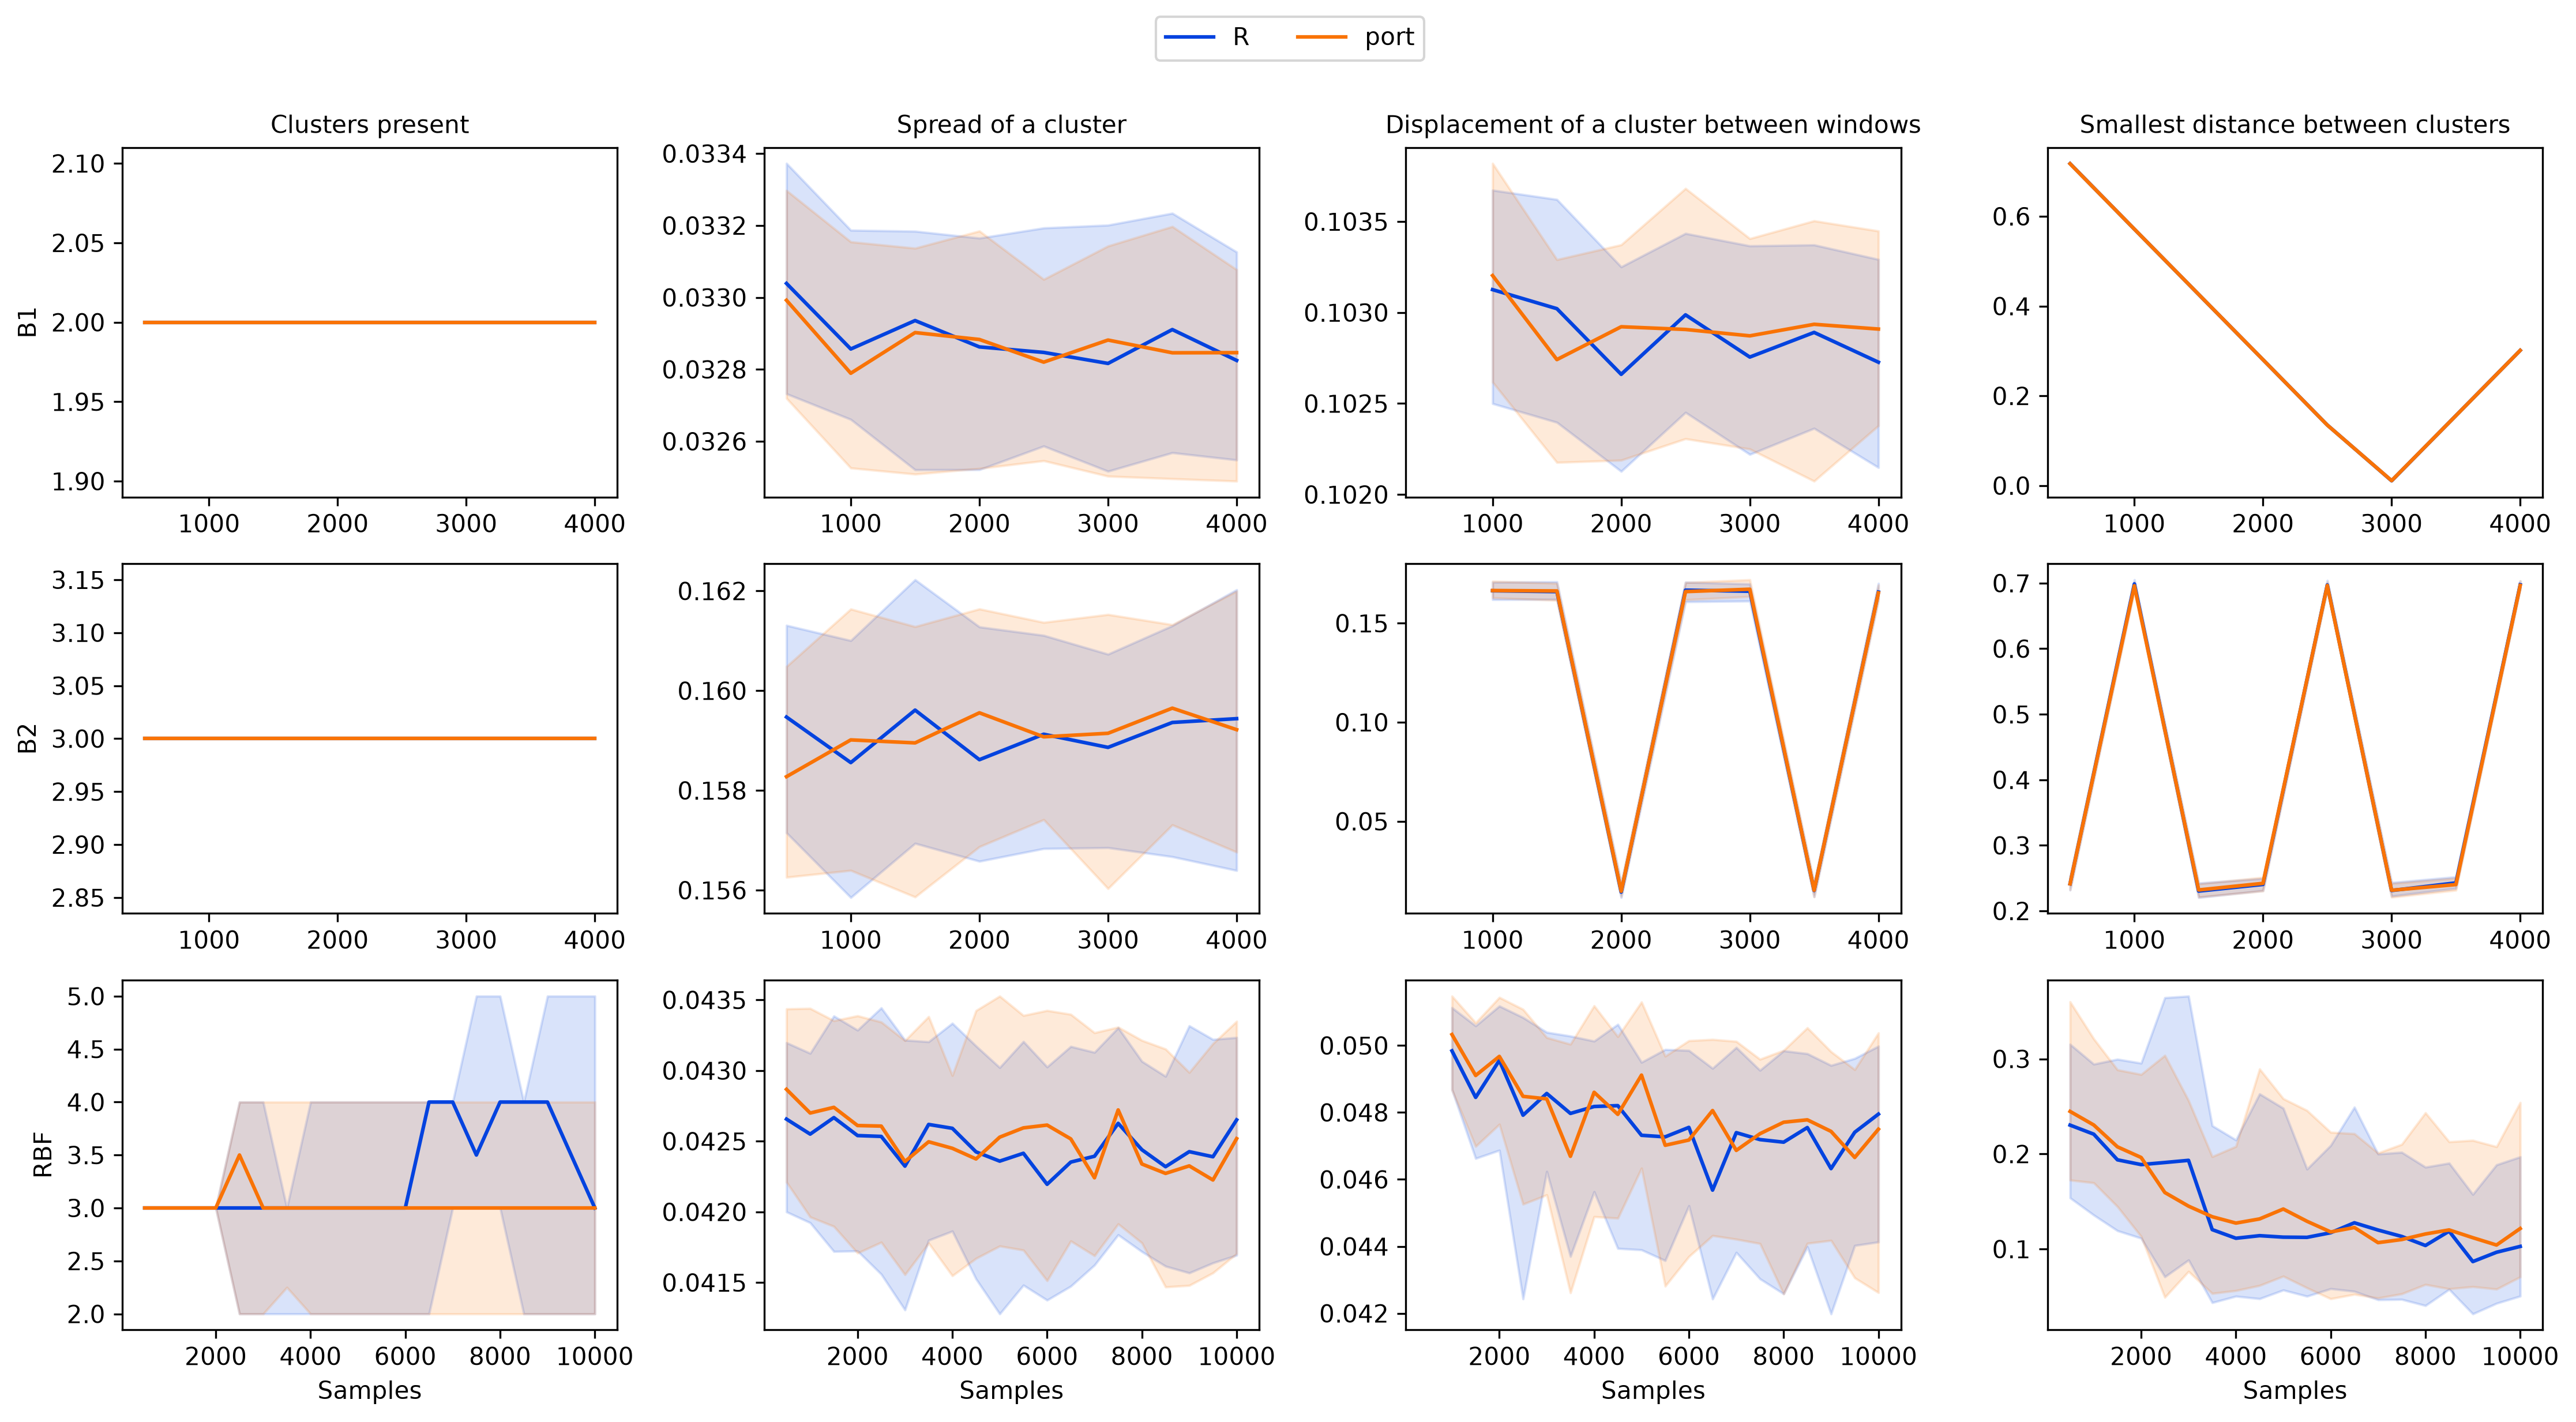
\includegraphics[width=\textwidth]{Modernization/artifacts/generators/plots/descriptors.png}
    \caption{Descriptors of the concept drift streams generated by \codename{R} and by the port, along the stream: medians and interquartile bands over the streams.}
    \label{fig:mod_generators_descriptors}
\end{figure}

\begin{table}[htbp]
\centering
\small
\caption[Models with fixed hyperparameters on the streams generated by R and by the port]{Models with fixed hyperparameters on the streams generated by R and by the port: medians over the streams. A value in red is significantly different from that of R.}
\adjustbox{max width=\textwidth, max totalheight=0.82\textheight}{%
\begin{tabular}{l c c c c }
\toprule
Model and source & B1 & B2 & RBF & CSN \\
\midrule
\multicolumn{5}{l}{\textit{Overall ARI}} \\
MicroTEDAClus+, R & 0.956 & 0.663 & 0.598 & 0.200 \\
MicroTEDAClus+, port & 0.953 & 0.666 & 0.617 & 0.197 \\
mini-batch k-means, R & 0.821 & 0.638 & 0.428 & 0.562 \\
mini-batch k-means, port & 0.816 & 0.647 & 0.431 & 0.540 \\
BIRCH, R & 0.132 & 0.691 & 0.377 & 1.000 \\
BIRCH, port & 0.133 & 0.688 & 0.366 & 1.000 \\
\midrule
\multicolumn{5}{l}{\textit{Steady-State ARI}} \\
MicroTEDAClus+, R & 0.973 & 0.783 & 0.599 & 0.171 \\
MicroTEDAClus+, port & 0.956 & 0.777 & 0.587 & 0.165 \\
mini-batch k-means, R & 0.832 & 0.832 & 0.376 & 0.571 \\
mini-batch k-means, port & 0.828 & 0.847 & 0.455 & 0.572 \\
BIRCH, R & 0.138 & 0.931 & 0.381 & 1.000 \\
BIRCH, port & 0.127 & 0.940 & 0.389 & 1.000 \\
\bottomrule
\end{tabular}
}
\label{tab:mod_generators_behaviour}
\end{table}


The interface through which the previous experiment generated \RandomRBFGeneratorEvents gives the noise the class value of the first cluster that the generator creates after the initial ones, so the samples of that cluster are labelled as noise. The port labels the noise apart from every cluster, and the comparisons above apply the labelling of the reference to both sources. \Cref{tab:mod_generators_rbf_noise} shows the share of samples labelled as noise along the stream under each labelling.

\begin{table}[htbp]
\centering
\small
\caption[Share of the samples of the Random RBF stream that carry the noise label]{Share of the samples of the Random RBF stream that carry the noise label, in consecutive blocks of 1000 samples: medians over the streams.}
\adjustbox{max width=\textwidth, max totalheight=0.82\textheight}{%
\begin{tabular}{l c c c c c c c c c c }
\toprule
Source & 1 & 2 & 3 & 4 & 5 & 6 & 7 & 8 & 9 & 10 \\
\midrule
R & 0.10 & 0.33 & 0.33 & 0.31 & 0.29 & 0.24 & 0.22 & 0.20 & 0.12 & 0.12 \\
port, labels of the R wrapper & 0.10 & 0.33 & 0.29 & 0.30 & 0.26 & 0.24 & 0.22 & 0.14 & 0.11 & 0.11 \\
port & 0.10 & 0.10 & 0.10 & 0.10 & 0.10 & 0.10 & 0.10 & 0.10 & 0.10 & 0.10 \\
\bottomrule
\end{tabular}
}
\label{tab:mod_generators_rbf_noise}
\end{table}


\subsection{Length and Order of the Streams}
\label{subsec:mod_streams}

The generated streams are five times longer than those of the previous experiment, and so are their tuning segments, in answer to \cref{sec:mi_selection}. The Chameleon files keep their size. The streams without concept drift, which are those of \Cassini, of the Chameleon datasets and of the scalability datasets, are shuffled anew in every run. Each run of a Chameleon dataset thus has a stream of its own, where in the previous experiment all its runs processed one same stream, \cref{subsec:mi_selection_consequences}. The concept drift streams keep their order, which carries the drift.

\section{Benchmark Models}
\label{sec:mod_models}

The benchmark models are chosen by three criteria: they are established in the literature of stream clustering, their implementations are maintained libraries that the experiment imports instead of copying, and they are fast enough to be tuned without a time limit. Five models are retained: \DenStream \cite{cao2006density} and \DBSTREAM \cite{hahsler2016dbstream}, from \codename{River} \cite{montiel2021river}; \BIRCH \cite{zhang1996birch} and \MiniBatchKMeans \cite{sculley2010webscale}, from \codename{scikit-learn} \cite{pedregosa2011scikit}; and \BICO \cite{fichtenberger2013bico}, from the \codename{bico} package. They summarize the stream by density-based microclusters that fade, \DenStream and \DBSTREAM, by a tree of cluster features, \BIRCH, by a coreset, \BICO, and by centroids, \MiniBatchKMeans. This set replaces that of \cref{chap:results}.

\Cref{tab:mod_hyperparameters} lists the hyperparameters that the search selects for each model. A parameter is searched if it is part of the clustering method, and keeps the default of its library if it only sets a unit of time or the shape of a data structure. \DenStream and \DBSTREAM forget at a rate that is searched as its half-life, in samples. The outlier threshold $\beta\mu$ of \DenStream, which its formulation requires to exceed one, is searched as its position between one and $\mu$.

\begin{table}[htbp]
\centering
\small
\caption[Hyperparameters of the models and their categories]{Hyperparameters that the search selects for each model, and the category that gives each its range.}
\adjustbox{max width=\textwidth, max totalheight=0.82\textheight}{%
\begin{tabular}{l l l}
\toprule
Model & Hyperparameter & Category \\
\midrule
\modelname{MicroTEDAClus+} & \texttt{variance\_limit} & Relative variance \\
 & \texttt{decay} & Horizon \\
 & \texttt{noise\_distance} & Multiplier \\
\midrule
\modelname{DenStream} & \texttt{epsilon} & Distance \\
 & \texttt{half\_life} & Horizon \\
 & \texttt{mu} & Minimum points \\
 & \texttt{outlier\_ratio} & Ratio \\
 & \texttt{n\_samples\_init} & Horizon \\
\midrule
\modelname{DBSTREAM} & \texttt{clustering\_threshold} & Distance \\
 & \texttt{half\_life} & Horizon \\
 & \texttt{cleanup\_interval} & Horizon \\
 & \texttt{intersection\_factor} & Ratio \\
 & \texttt{minimum\_weight} & Minimum points \\
\midrule
\modelname{BIRCH} & \texttt{threshold} & Distance \\
 & \texttt{n\_clusters} & Clusters \\
\midrule
\modelname{Mini-batch k-means} & \texttt{n\_clusters} & Clusters \\
 & \texttt{reassignment\_ratio} & Ratio \\
\midrule
\modelname{BICO} & \texttt{n\_clusters} & Clusters \\
 & \texttt{summary\_size} & Summary size \\
\bottomrule
\end{tabular}
}
\label{tab:mod_hyperparameters}
\end{table}


\section{Hyperparameter Selection}
\label{sec:mod_selection}

The search remains the Bayesian optimization of \cref{subsec:hyperparameter_tuning} on the first 20\% of each stream, and the selected model is evaluated prequentially on the rest. Three things change: where the ranges come from, what the objective measures, and what bounds the search.

\subsection{Ranges by Rule}
\label{subsec:mod_ranges}

Each hyperparameter belongs to a kind, given in \cref{tab:mod_hyperparameters}, and each kind has one rule that computes its range from the tuning segment, given in \cref{tab:mod_rules}. A rule uses only what a deployment of the model also has before the stream continues: the samples of the segment and their labels. Below the median distance from a sample to its nearest neighbour, a structure of that radius holds a single sample, and above the median distance between two samples it holds half of the segment, so the distances of the rules span the scales at which a structure can summarize the data. The longest horizon is the length of the segment, the longest that the segment can tell apart from not forgetting at all. The rules replace ranges set by hand, which \cref{tab:mi_search_range_selection} showed to depend on the scale of the data. \Cref{tab:mod_ranges} gives the ranges that they produce in each dataset.

\begin{table}[htbp]
\centering
\caption{Rule of each kind of hyperparameter, for a tuning segment of $n$ samples with $k$ labelled clusters. Horizons, summary sizes, minimum points and numbers of clusters are integers.}
\begin{tabular}{p{0.16\textwidth} p{0.29\textwidth} p{0.29\textwidth} l}
\toprule
Kind & Lower end & Upper end & Scale \\
\midrule
Distance & median distance from a sample to its nearest neighbour & median distance between two samples & logarithmic \\
Relative variance & square of the lower distance, as a fraction of the total variance & square of the upper distance, as a fraction of the total variance & logarithmic \\
Horizon & $n/100$ samples & $n$ samples & logarithmic \\
Summary size & $2k$ & $n/4$ & logarithmic \\
Minimum points & $2$ & $\sqrt{n}$ & logarithmic \\
Ratio & $0.01$ & $0.99$ & linear \\
Multiplier & $1$ & $10$ & linear \\
Clusters & $2$ & $2k$ & linear \\
\bottomrule
\end{tabular}
\label{tab:mod_rules}
\end{table}

\begin{table}[htbp]
\centering
\small
\caption[Search ranges that the rules give]{Search ranges that the rules give to each category of hyperparameter: medians over 94 runs of the two ends of each range.}
\adjustbox{max width=\textwidth, max totalheight=0.82\textheight}{%
\begin{tabular}{l c c c c c c }
\toprule
Dataset & Distance & Relative variance & Horizon & Summary size & Minimum points & Clusters \\
\midrule
B1 & $2.1 \times 10^{-4}$ to 3.3 & $5.5 \times 10^{-7}$ to 138 & 4 to 4000 & 4 to 1000 & 1 to 63 & 2 to 40 \\
B2 & $5.3 \times 10^{-4}$ to 6.5 & $7.0 \times 10^{-7}$ to 106 & 4 to 4000 & 6 to 1000 & 1 to 63 & 2 to 60 \\
RBF & $2.5 \times 10^{-4}$ to 3.2 & $7.8 \times 10^{-7}$ to 136 & 10 to 10000 & 16 to 2500 & 1 to 100 & 2 to 100 \\
CSN & 0.002 to 16 & $2.2 \times 10^{-6}$ to 142 & 4 to 4000 & 6 to 1000 & 1 to 63 & 2 to 60 \\
DS3 & 0.44 to 2802 & $3.5 \times 10^{-6}$ to 146 & 2 to 2000 & 18 to 500 & 1 to 45 & 2 to 100 \\
DS4 & 0.48 to 2598 & $4.9 \times 10^{-6}$ to 143 & 2 to 1600 & 16 to 400 & 1 to 40 & 2 to 100 \\
S1 & $4.9 \times 10^{-5}$ to 30 & $1.2 \times 10^{-10}$ to 65 & 5 to 4400 & 6 to 1100 & 1 to 66 & 2 to 60 \\
S2 & 0.0026 to 60 & $1.8 \times 10^{-7}$ to 106 & 5 to 4400 & 6 to 1100 & 1 to 66 & 2 to 60 \\
S4 & 0.021 to 113 & $4.9 \times 10^{-6}$ to 167 & 5 to 4400 & 6 to 1100 & 1 to 66 & 2 to 60 \\
S8 & 0.067 to 195 & $2.5 \times 10^{-5}$ to 216 & 5 to 4400 & 6 to 1100 & 1 to 66 & 2 to 60 \\
S16 & 0.15 to 285 & $6.0 \times 10^{-5}$ to 230 & 5 to 4400 & 6 to 1100 & 1 to 66 & 2 to 60 \\
S32 & 0.26 to 419 & $9.7 \times 10^{-5}$ to 252 & 5 to 4400 & 6 to 1100 & 1 to 66 & 2 to 60 \\
S64 & 0.43 to 612 & $1.3 \times 10^{-4}$ to 270 & 5 to 4400 & 6 to 1100 & 1 to 66 & 2 to 60 \\
\bottomrule
\end{tabular}
}
\label{tab:mod_ranges}
\end{table}


\subsection{Objective and Search}
\label{subsec:mod_objective}

The objective is the median of the batch ARI over the second half of the tuning segment. It is the quantity that the Overall ARI reports, computed after the configuration has had the first half of the segment to form its summary, which addresses the slow maturation shown in \cref{tab:mi_selection_maturation}. It has no term of execution time.

Every model receives 100 trials, without a time limit. The search of a task is seeded by its dataset, its model and its run, and its objective involves no measurement of time, so the selection depends neither on the speed of the machine nor on its load. To measure what the change of protocol does, \MicroTEDAClusPlus is also tuned by the previous protocol of \cref{subsec:hyperparameter_tuning}, with its previous ranges, on the same streams.

\section{Execution and Measurements}
\label{sec:mod_measurements}

A task is a dataset, a model and a run, and the experiment executes the tasks of 94 runs, 13 datasets and the six models in parallel processes. Parallel execution disturbs the execution time, so time is measured in a separate pass: the tasks of the first ten runs are evaluated again, one at a time, with their selected hyperparameters, three times each, and the fastest evaluation is kept.

Memory is measured in another pass, over every task, by tracking every allocation of the process with \codename{memray} \cite{memray}, which counts the memory allocated by compiled code as well as that allocated by \codename{Python}. Two quantities are kept: the memory still allocated when the stream ends, which is what the model holds, and the peak during the evaluation, which adds the working memory of its steps. Each task is first evaluated without tracking, so that what is created on first use is in place, and then tracked three times, of which the smallest values are kept. These quantities are not comparable with the memory reported in the previous chapters, which counted only the \codename{Python} objects of a model.

The results are compared by the analysis of \cref{sec:statistical_significance}, as in \cref{chap:results}: a value in bold is statistically indistinguishable from the best model of its dataset, and a value in red from the worst. The tables refer to the datasets by the abbreviations of \cref{tab:mi_dataset_abbreviations}, and to \datasetname{SCL-$d$} as S$d$.

\section{Results}
\label{sec:mod_results}

\subsection{Clustering Quality}
\label{subsec:mod_quality}

\begin{table}[htbp]
\centering
\small
\caption[Clustering quality of \modelname{MicroTEDAClus+} and the benchmark models]{Clustering quality of \modelname{MicroTEDAClus+} and the benchmark models: medians over 94 runs.}
\adjustbox{max width=\textwidth, max totalheight=0.82\textheight}{%
\begin{tabular}{l c c c c c c }
\toprule
Model & B1 & B2 & RBF & CSN & DS3 & DS4 \\
\midrule
\multicolumn{7}{l}{\textit{Overall ARI}} \\
\modelname{MicroTEDAClus+} & 0.889 & 0.599 & 0.653 & 0.916 & 0.347 & 0.378 \\
Better/same/worse & 5/0/0 & 0/0/5 & 1/1/3 & 4/1/0 & 0/4/1 & 2/3/0 \\
\modelname{DenStream} & \textbf{0.829} & \textcolor{red}{0.625} & 0.605 & \textbf{0.637} & 0.381 & \textbf{0.354} \\
\modelname{DBSTREAM} & \textbf{0.852} & \textcolor{red}{0.825} & \textcolor{red}{0.664} & \textbf{0.758} & 0.371 & \textbf{0.354} \\
\modelname{BIRCH} & \textbf{0.821} & \textcolor{red}{0.673} & \textcolor{red}{0.690} & 1.000 & 0.356 & 0.378 \\
\modelname{Mini-batch k-means} & \textbf{0.863} & \textcolor{red}{0.642} & \textbf{0.587} & \textbf{0.588} & 0.377 & 0.366 \\
\modelname{BICO} & \textbf{0.876} & \textcolor{red}{0.774} & \textcolor{red}{0.681} & \textbf{0.595} & \textcolor{red}{0.409} & 0.371 \\
\midrule
\multicolumn{7}{l}{\textit{Steady-State ARI}} \\
\modelname{MicroTEDAClus+} & 0.790 & 0.567 & 0.466 & 0.792 & 0.348 & 0.367 \\
Better/same/worse & 4/1/0 & 0/0/5 & 0/0/5 & 2/2/1 & 0/4/1 & 0/5/0 \\
\modelname{DenStream} & \textbf{0.718} & \textcolor{red}{0.637} & \textcolor{red}{0.621} & 0.686 & 0.380 & 0.354 \\
\modelname{DBSTREAM} & 0.859 & \textcolor{red}{0.790} & \textcolor{red}{0.760} & 0.786 & 0.362 & 0.352 \\
\modelname{BIRCH} & \textbf{0.136} & \textcolor{red}{0.714} & \textcolor{red}{0.677} & \textcolor{red}{1.000} & 0.378 & 0.365 \\
\modelname{Mini-batch k-means} & \textbf{0.611} & \textcolor{red}{0.663} & \textcolor{red}{0.609} & \textbf{0.599} & 0.391 & 0.356 \\
\modelname{BICO} & \textbf{0.180} & \textcolor{red}{0.758} & \textcolor{red}{0.718} & \textbf{0.596} & \textcolor{red}{0.406} & 0.359 \\
\bottomrule
\end{tabular}
}
\label{tab:mod_quality}
\end{table}


In the Overall ARI, \cref{tab:mod_quality}, \MicroTEDAClusPlus is indistinguishable from the best model in \BenchmarkOne, \Cassini and \ChameleonDSFour, and from the worst in \BenchmarkTwo and \ChameleonDSThree. At the penultimate batch, \DBSTREAM is indistinguishable from the best model in the three concept drift datasets, and \MicroTEDAClusPlus in \BenchmarkOne only. At the fifth batch, \MicroTEDAClusPlus is indistinguishable from the best model in the three concept drift datasets and from the worst in the three static ones.

In \BenchmarkOne, \BIRCH and \BICO have the largest drops of the table and the lowest scores at the penultimate batch. Neither of them forgets, and the clusters of that stream move.

\begin{table}[htbp]
\centering
\caption{Quality of the models along the dimension of the data: medians over 94 runs. A value in bold is statistically indistinguishable from the best model of its dataset, and a value in red from the worst.}
\adjustbox{width=\textwidth, totalheight=0.82\textheight, keepaspectratio}{%
\begin{tabular}{l c c c c c c c }
\toprule
Model & S1 & S2 & S4 & S8 & S16 & S32 & S64 \\
\midrule
\multicolumn{8}{l}{\textit{Overall ARI}} \\
\modelname{MicroTEDAClus+} & \textcolor{red}{0.719} & \textbf{0.938} & \textbf{1.000} & \textbf{1.000} & \textbf{1.000} & \textbf{1.000} & \textbf{1.000} \\
\modelname{DenStream} & 0.780 & 0.885 & 0.961 & 0.968 & \textcolor{red}{0.978} & \textcolor{red}{0.991} & 1.000 \\
\modelname{DBSTREAM} & \textbf{0.776} & 0.928 & 0.966 & 0.975 & \textcolor{red}{0.975} & \textcolor{red}{0.982} & 0.986 \\
\modelname{BIRCH} & \textbf{0.806} & 0.923 & 0.951 & 1.000 & \textbf{1.000} & 1.000 & \textcolor{red}{0.895} \\
\modelname{Mini-batch k-means} & \textbf{0.779} & \textcolor{red}{0.855} & \textcolor{red}{0.901} & \textcolor{red}{0.948} & \textcolor{red}{0.981} & 1.000 & 1.000 \\
\modelname{BICO} & \textbf{0.800} & 0.891 & 0.940 & 0.963 & 0.982 & \textbf{1.000} & 1.000 \\
\midrule
\multicolumn{8}{l}{\textit{Steady-State ARI}} \\
\modelname{MicroTEDAClus+} & \textcolor{red}{0.698} & \textbf{0.925} & \textbf{0.998} & \textbf{1.000} & \textbf{1.000} & \textbf{1.000} & \textbf{1.000} \\
\modelname{DenStream} & 0.748 & 0.875 & 0.957 & 0.968 & \textcolor{red}{0.972} & \textcolor{red}{0.999} & 1.000 \\
\modelname{DBSTREAM} & \textbf{0.776} & \textbf{0.917} & 0.971 & 0.974 & \textcolor{red}{0.972} & \textcolor{red}{0.981} & 0.984 \\
\modelname{BIRCH} & \textbf{0.792} & \textbf{0.913} & 0.954 & 1.000 & \textbf{1.000} & 1.000 & \textcolor{red}{0.881} \\
\modelname{Mini-batch k-means} & \textbf{0.795} & \textcolor{red}{0.849} & \textcolor{red}{0.902} & \textcolor{red}{0.946} & 0.982 & 1.000 & \textbf{1.000} \\
\modelname{BICO} & \textbf{0.758} & 0.888 & 0.933 & 0.965 & 0.983 & \textbf{1.000} & \textbf{1.000} \\
\bottomrule
\end{tabular}
}
\label{tab:mod_scalability}
\end{table}


\begin{figure}[htbp]
    \centering
    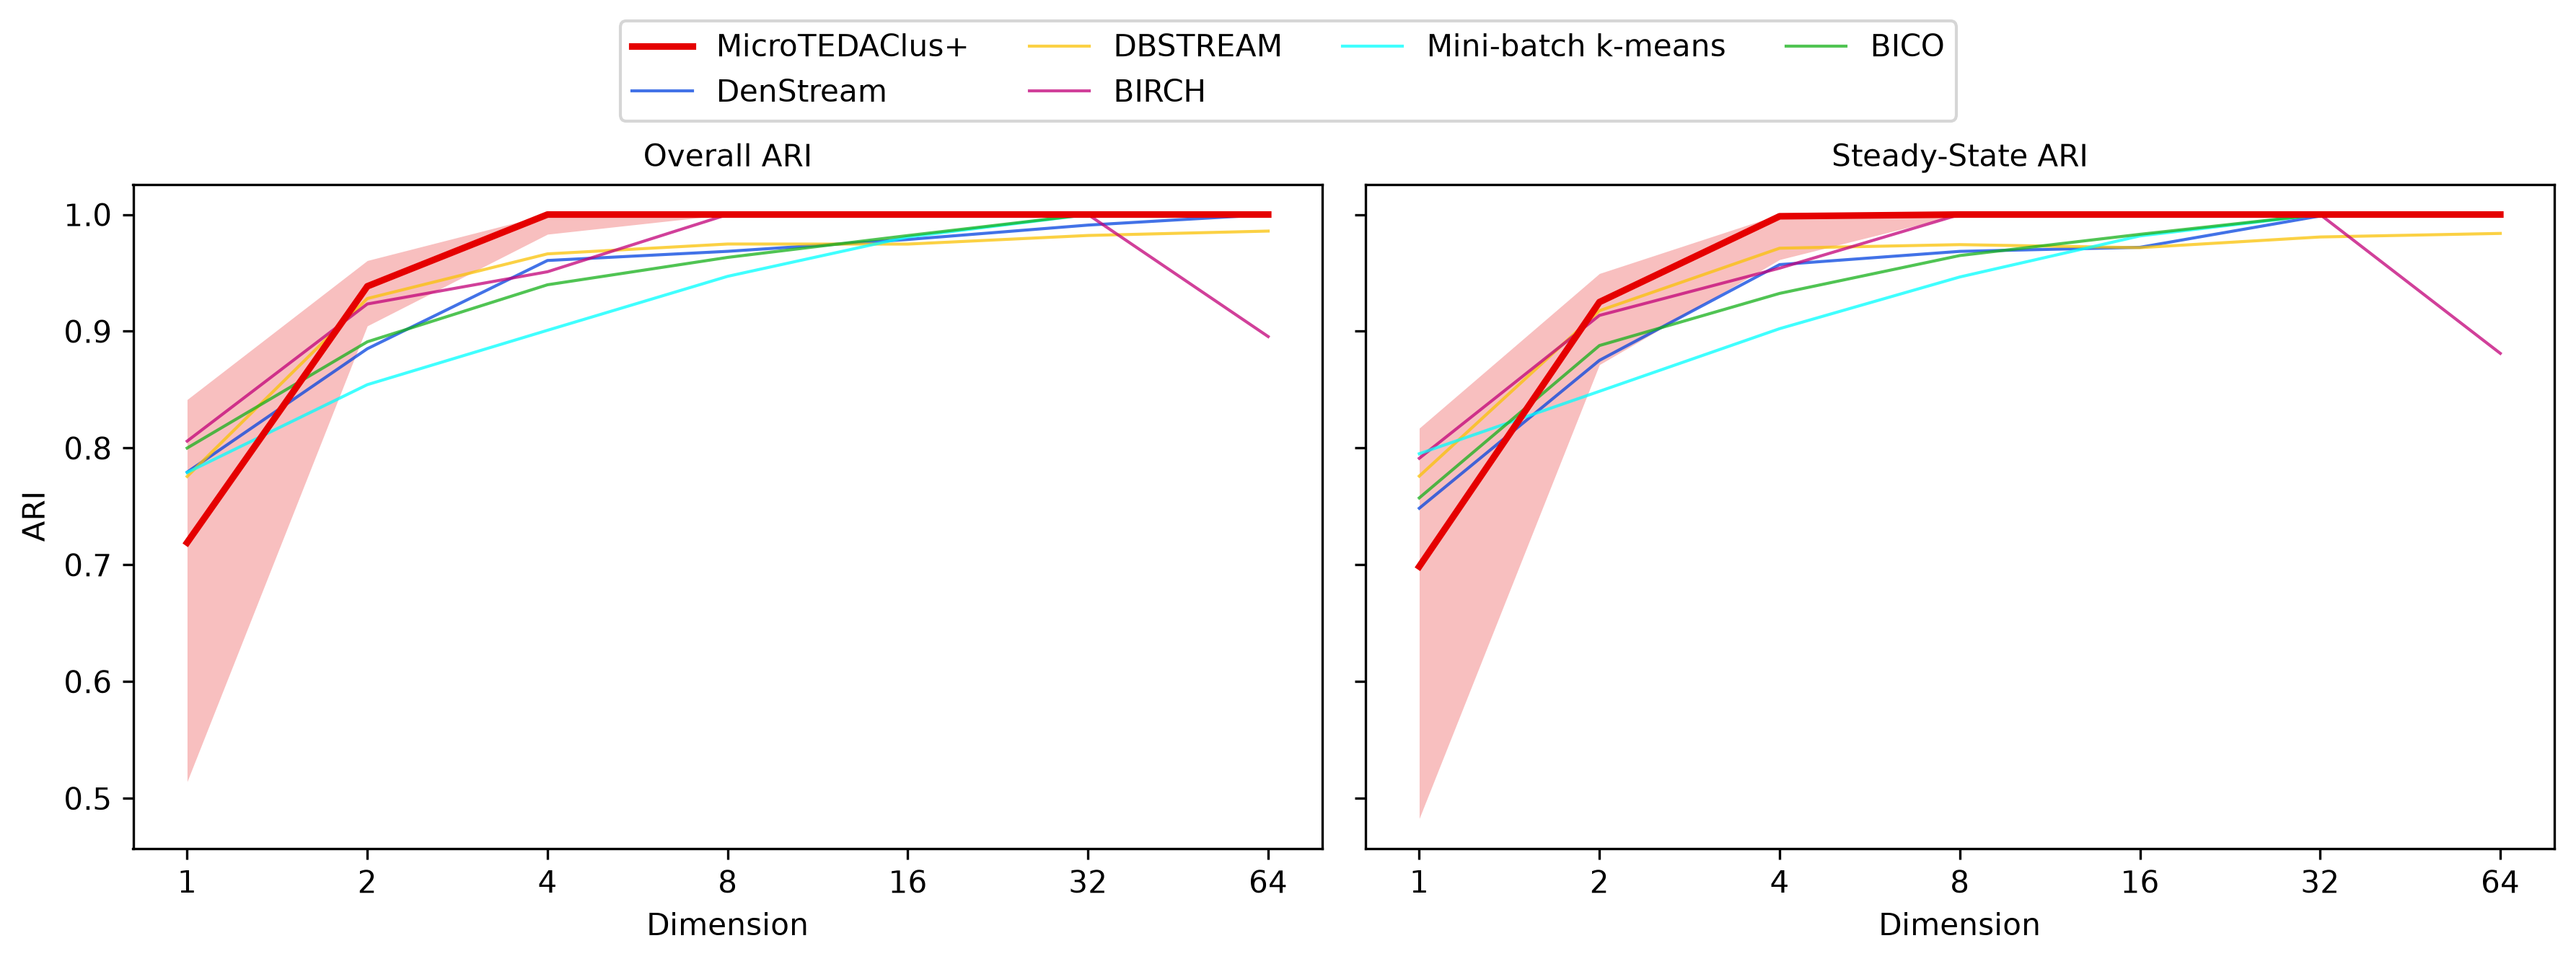
\includegraphics[width=\textwidth]{Modernization/artifacts/experiment/plots/dimension_scalability.png}
    \caption{ARI at the fifth batch, at left, and at the penultimate batch, at right, against the dimension of the scalability streams: medians and interquartile bands over 94 runs.}
    \label{fig:mod_dimension}
\end{figure}

In the scalability streams, \cref{tab:mod_scalability,fig:mod_dimension}, \MicroTEDAClusPlus is indistinguishable from the best model from two dimensions on, in both metrics, and from the worst with one dimension. \BIRCH, among the best with sixteen dimensions, is among the worst with sixty-four, where its score varies widely along the stream, \cref{fig:mod_stream}.

\begin{figure}[htbp]
    \centering
    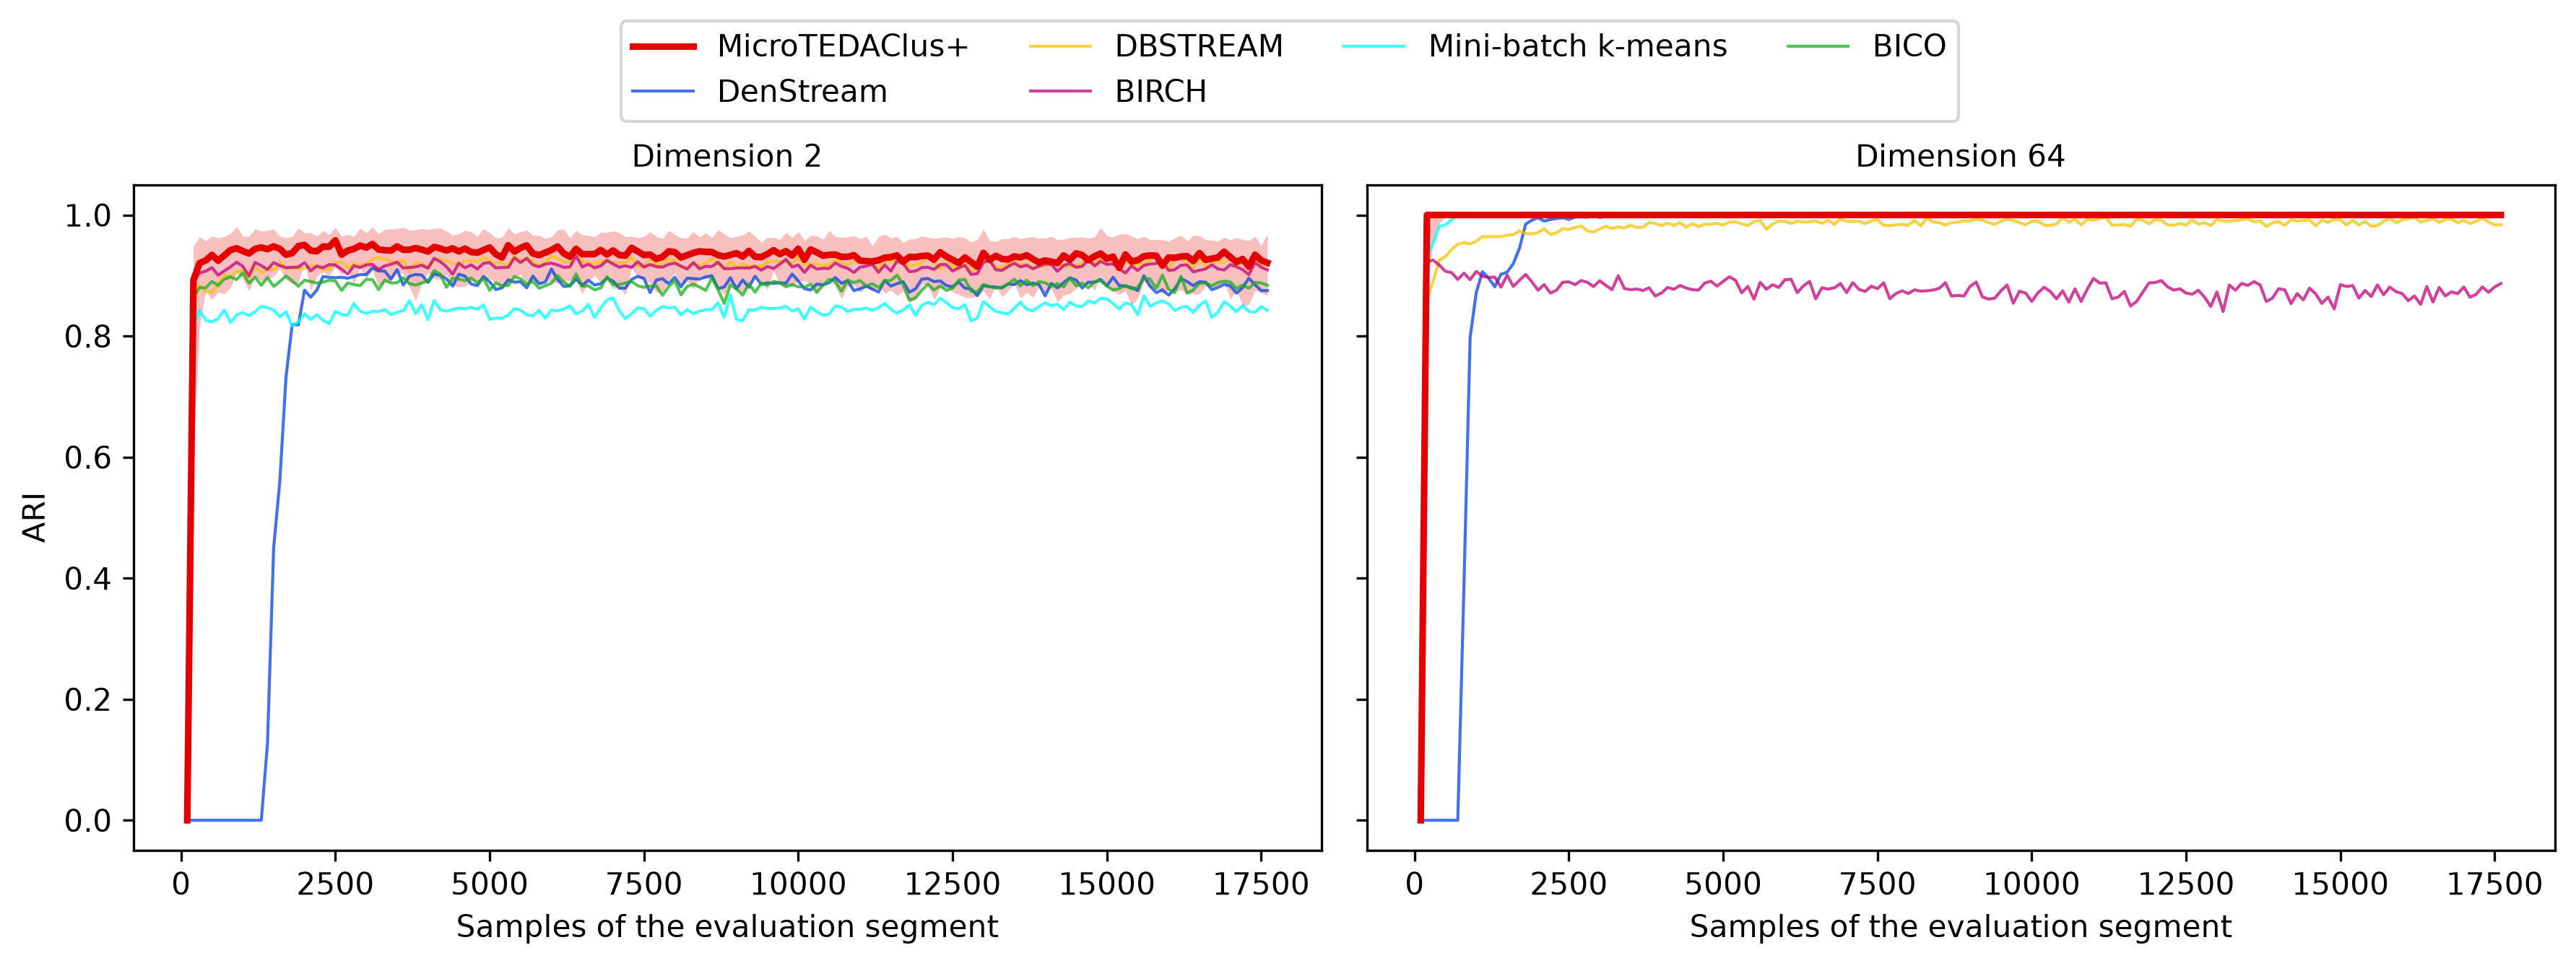
\includegraphics[width=\textwidth]{Modernization/artifacts/experiment/plots/stream_scalability.png}
    \caption{Batch ARI along the evaluation segment of \datasetname{SCL-2}, at left, and of \datasetname{SCL-64}, at right: medians and interquartile bands over 94 runs.}
    \label{fig:mod_stream}
\end{figure}

\DenStream scores zero at the fifth batch in the concept drift datasets, \cref{tab:mod_quality}, and from two dimensions on, \cref{fig:mod_dimension}. \Cref{fig:mod_stream} shows why: it labels every sample as noise until its initialization buffer is full, and the search selects long buffers. The objective scores only the second half of the tuning segment, where a late start costs nothing, while the Overall ARI counts the whole stream. This disagreement between the objective and the reported metric is a limitation of the protocol, not of the model, and the experiment was not repeated without it.

\subsection{The Change of Protocol}
\label{subsec:mod_protocols}

\begin{table}[htbp]
\centering
\small
\caption[\MicroTEDAClusPlus{} under the two protocols of hyperparameter selection]{\MicroTEDAClusPlus{} with its hyperparameters selected by the previous protocol and by the protocol by rules, on the same streams: medians over 94 runs.}
\adjustbox{max width=\textwidth, max totalheight=0.82\textheight}{%
\begin{tabular}{l c c c c c c c c c c c c c }
\toprule
Selection & B1 & B2 & RBF & CSN & DS3 & DS4 & S1 & S2 & S4 & S8 & S16 & S32 & S64 \\
\midrule
\multicolumn{14}{l}{\textit{Overall ARI}} \\
Previous protocol & 0.897 & 0.605 & 0.573 & 0.607 & 0.295 & 0.345 & 0.702 & 0.942 & 1.000 & 1.000 & 1.000 & 1.000 & 1.000 \\
Protocol by rules & 0.889 & \textcolor{red}{0.599} & \textbf{0.653} & \textbf{0.916} & \textbf{0.347} & \textbf{0.378} & 0.719 & 0.938 & 1.000 & 1.000 & 1.000 & \textbf{1.000} & \textbf{1.000} \\
\midrule
\multicolumn{14}{l}{\textit{Steady-State ARI}} \\
Previous protocol & 0.223 & 0.573 & 0.215 & 0.421 & 0.279 & 0.324 & 0.595 & 0.924 & 0.998 & 1.000 & 1.000 & 1.000 & 1.000 \\
Protocol by rules & \textbf{0.790} & 0.567 & 0.466 & \textbf{0.792} & \textbf{0.348} & \textbf{0.367} & 0.698 & 0.925 & 0.998 & 1.000 & 1.000 & \textbf{1.000} & 1.000 \\
\bottomrule
\end{tabular}
}
\label{tab:mod_protocols}
\end{table}


\Cref{tab:mod_protocols} compares \MicroTEDAClusPlus under the two protocols on the same streams. The protocol by rules raises its Overall ARI in six datasets and lowers it in \BenchmarkTwo, and raises its Steady-State ARI in five datasets without lowering it in any. The largest differences are at the penultimate batch of \BenchmarkOne and \Cassini. This agrees with \cref{subsec:mi_selection_consequences}, which located the most direct improvement of the model in the selection of its hyperparameters rather than in its algorithm.

\subsection{Selected Hyperparameters}
\label{subsec:mod_selected}

\begin{table}[htbp]
\centering
\small
\caption[Selected values at the ends of their search ranges]{Percentage of the 94 runs in which the selected value of a hyperparameter lies within a twentieth of the width of its search range from one of its ends, in the scale of the search.}
\adjustbox{max width=\textwidth, max totalheight=0.82\textheight}{%
\begin{tabular}{l c c c c c c c c c c c c c }
\toprule
Model and hyperparameter & B1 & B2 & RBF & CSN & DS3 & DS4 & S1 & S2 & S4 & S8 & S16 & S32 & S64 \\
\midrule
\multicolumn{14}{l}{\textit{At the lower end}} \\
\modelname{MicroTEDAClus+}, \texttt{variance\_limit} & 0 & 0 & 0 & 0 & 0 & 0 & 0 & 0 & 6 & 13 & 4 & 6 & 3 \\
\modelname{MicroTEDAClus+}, \texttt{decay} & 31 & 13 & 16 & 0 & 4 & 3 & 3 & 1 & 5 & 2 & 3 & 2 & 4 \\
\modelname{MicroTEDAClus+}, \texttt{noise\_distance} & 0 & 0 & 0 & 0 & 0 & 0 & 0 & 0 & 0 & 0 & 2 & 0 & 3 \\
\modelname{DenStream}, \texttt{epsilon} & 7 & 2 & 0 & 0 & 0 & 2 & 0 & 3 & 0 & 0 & 1 & 1 & 1 \\
\modelname{DenStream}, \texttt{half\_life} & 0 & 1 & 6 & 0 & 2 & 9 & 2 & 1 & 1 & 1 & 7 & 7 & 4 \\
\modelname{DenStream}, \texttt{mu} & 46 & 4 & 18 & 1 & 17 & 14 & 21 & 29 & 69 & 52 & 18 & 15 & 14 \\
\modelname{DenStream}, \texttt{outlier\_ratio} & 6 & 10 & 4 & 6 & 3 & 3 & 7 & 6 & 3 & 4 & 4 & 5 & 5 \\
\modelname{DenStream}, \texttt{n\_samples\_init} & 0 & 3 & 1 & 13 & 0 & 1 & 3 & 3 & 0 & 1 & 1 & 0 & 1 \\
\modelname{DBSTREAM}, \texttt{clustering\_threshold} & 0 & 0 & 0 & 0 & 0 & 0 & 0 & 0 & 0 & 0 & 0 & 0 & 1 \\
\modelname{DBSTREAM}, \texttt{half\_life} & 0 & 3 & 19 & 1 & 3 & 3 & 5 & 1 & 0 & 0 & 0 & 0 & 3 \\
\modelname{DBSTREAM}, \texttt{cleanup\_interval} & 6 & 3 & 4 & 2 & 4 & 5 & 6 & 2 & 2 & 3 & 5 & 5 & 5 \\
\modelname{DBSTREAM}, \texttt{intersection\_factor} & 3 & 0 & 2 & 1 & 2 & 5 & 6 & 5 & 2 & 1 & 1 & 7 & 2 \\
\modelname{DBSTREAM}, \texttt{minimum\_weight} & 19 & 13 & 27 & 11 & 18 & 15 & 13 & 32 & 50 & 44 & 40 & 18 & 15 \\
\modelname{BIRCH}, \texttt{threshold} & 1 & 3 & 16 & 6 & 6 & 7 & 9 & 23 & 51 & 70 & 73 & 90 & 9 \\
\modelname{BIRCH}, \texttt{n\_clusters} & 16 & 0 & 0 & 0 & 0 & 0 & 3 & 0 & 0 & 0 & 0 & 0 & 0 \\
\modelname{Mini-batch k-means}, \texttt{n\_clusters} & 3 & 0 & 0 & 5 & 0 & 0 & 9 & 0 & 0 & 0 & 0 & 0 & 0 \\
\modelname{Mini-batch k-means}, \texttt{reassignment\_ratio} & 1 & 7 & 19 & 3 & 7 & 5 & 28 & 46 & 59 & 51 & 48 & 29 & 20 \\
\modelname{BICO}, \texttt{n\_clusters} & 15 & 0 & 0 & 1 & 0 & 0 & 5 & 0 & 0 & 0 & 0 & 0 & 0 \\
\modelname{BICO}, \texttt{summary\_size} & 11 & 1 & 1 & 12 & 1 & 2 & 4 & 0 & 1 & 2 & 1 & 0 & 0 \\
\midrule
\multicolumn{14}{l}{\textit{At the upper end}} \\
\modelname{MicroTEDAClus+}, \texttt{variance\_limit} & 0 & 0 & 0 & 0 & 0 & 0 & 34 & 5 & 1 & 4 & 5 & 4 & 5 \\
\modelname{MicroTEDAClus+}, \texttt{decay} & 0 & 0 & 0 & 15 & 18 & 7 & 11 & 7 & 3 & 4 & 6 & 7 & 3 \\
\modelname{MicroTEDAClus+}, \texttt{noise\_distance} & 24 & 2 & 4 & 9 & 10 & 5 & 0 & 2 & 2 & 0 & 0 & 3 & 1 \\
\modelname{DenStream}, \texttt{epsilon} & 1 & 2 & 10 & 14 & 4 & 5 & 28 & 3 & 0 & 1 & 2 & 2 & 1 \\
\modelname{DenStream}, \texttt{half\_life} & 4 & 7 & 1 & 3 & 5 & 6 & 3 & 6 & 6 & 4 & 3 & 5 & 9 \\
\modelname{DenStream}, \texttt{mu} & 0 & 10 & 1 & 3 & 0 & 1 & 6 & 1 & 0 & 0 & 0 & 2 & 2 \\
\modelname{DenStream}, \texttt{outlier\_ratio} & 3 & 5 & 2 & 4 & 3 & 6 & 5 & 4 & 4 & 3 & 3 & 5 & 5 \\
\modelname{DenStream}, \texttt{n\_samples\_init} & 0 & 0 & 0 & 0 & 0 & 0 & 0 & 0 & 0 & 0 & 0 & 0 & 0 \\
\modelname{DBSTREAM}, \texttt{clustering\_threshold} & 0 & 61 & 9 & 27 & 62 & 11 & 22 & 6 & 2 & 0 & 3 & 5 & 3 \\
\modelname{DBSTREAM}, \texttt{half\_life} & 16 & 9 & 3 & 5 & 7 & 6 & 4 & 10 & 11 & 20 & 16 & 9 & 7 \\
\modelname{DBSTREAM}, \texttt{cleanup\_interval} & 3 & 7 & 5 & 1 & 10 & 2 & 6 & 3 & 5 & 11 & 5 & 4 & 6 \\
\modelname{DBSTREAM}, \texttt{intersection\_factor} & 9 & 23 & 1 & 0 & 9 & 4 & 3 & 3 & 14 & 34 & 16 & 19 & 5 \\
\modelname{DBSTREAM}, \texttt{minimum\_weight} & 14 & 1 & 0 & 6 & 5 & 5 & 3 & 0 & 0 & 0 & 0 & 3 & 4 \\
\modelname{BIRCH}, \texttt{threshold} & 53 & 0 & 0 & 0 & 0 & 0 & 3 & 0 & 0 & 0 & 0 & 0 & 0 \\
\modelname{BIRCH}, \texttt{n\_clusters} & 53 & 1 & 26 & 0 & 0 & 1 & 12 & 79 & 62 & 5 & 2 & 15 & 94 \\
\modelname{Mini-batch k-means}, \texttt{n\_clusters} & 96 & 0 & 5 & 0 & 0 & 0 & 0 & 12 & 30 & 30 & 12 & 24 & 33 \\
\modelname{Mini-batch k-means}, \texttt{reassignment\_ratio} & 3 & 5 & 0 & 1 & 0 & 1 & 4 & 4 & 2 & 0 & 0 & 0 & 0 \\
\modelname{BICO}, \texttt{n\_clusters} & 85 & 0 & 21 & 0 & 0 & 0 & 1 & 62 & 97 & 73 & 12 & 0 & 6 \\
\modelname{BICO}, \texttt{summary\_size} & 5 & 12 & 9 & 1 & 7 & 7 & 5 & 3 & 2 & 7 & 4 & 10 & 5 \\
\bottomrule
\end{tabular}
}
\label{tab:mod_ends}
\end{table}


\Cref{tab:mod_ends} shows how often the selected value of each hyperparameter lies at an end of its range. For several hyperparameters of the benchmark models it does in a large share of the runs: the number of clusters of \MiniBatchKMeans, \BICO and \BIRCH at its upper end in \BenchmarkOne and in scalability streams, the threshold of \BIRCH at its lower end in the scalability streams from four to thirty-two dimensions, the threshold of \DBSTREAM at its upper end in \BenchmarkTwo and \ChameleonDSThree, the minimum weight of \DBSTREAM and the $\mu$ of \DenStream at their lower end, and the reassignment ratio of \MiniBatchKMeans at its lower end. The searches of these models were bounded by the rules, and wider ranges could change their results. The hyperparameters of \MicroTEDAClusPlus reach an end of their ranges less often. The experiment was not repeated with wider ranges.

\subsection{Cost}
\label{subsec:mod_cost}

\begin{table}[htbp]
\centering
\caption{Execution time of the models, each task measured alone: medians over 10 runs. A value in bold is statistically indistinguishable from the best model of its dataset, and a value in red from the worst.}
\adjustbox{width=\textwidth, totalheight=0.82\textheight, keepaspectratio}{%
\begin{tabular}{l c c c c c c c c c c c c c }
\toprule
Model & B1 & B2 & RBF & CSN & DS3 & DS4 & S1 & S2 & S4 & S8 & S16 & S32 & S64 \\
\midrule
\multicolumn{14}{l}{\textit{Learning time of the evaluation segment, in milliseconds}} \\
\modelname{MicroTEDAClus+} & 80.0 & 55.0 & \textbf{185.0} & 355.0 & \textcolor{red}{90.0} & 30.0 & 75.0 & 80.0 & 185.0 & 65.0 & 70.0 & 245.0 & 95.0 \\
\modelname{DenStream} & 175.0 & 40.0 & \textbf{140.0} & 40.0 & 20.0 & 20.0 & 40.0 & 60.0 & 95.0 & 105.0 & 150.0 & 240.0 & \textcolor{red}{440.0} \\
\modelname{DBSTREAM} & \textcolor{red}{805.0} & 60.0 & \textcolor{red}{500.0} & 95.0 & 50.0 & 65.0 & 100.0 & 270.0 & 455.0 & 590.0 & 650.0 & 525.0 & \textcolor{red}{605.0} \\
\modelname{BIRCH} & 200.0 & \textcolor{red}{270.0} & \textcolor{red}{715.0} & \textcolor{red}{1630.0} & \textcolor{red}{105.0} & \textcolor{red}{80.0} & \textcolor{red}{210.0} & \textcolor{red}{11500.0} & \textcolor{red}{22015.0} & \textcolor{red}{18035.0} & \textcolor{red}{13565.0} & \textcolor{red}{4210.0} & \textcolor{red}{2480.0} \\
\modelname{Mini-batch k-means} & 60.0 & 60.0 & \textbf{150.0} & 60.0 & 30.0 & 25.0 & 65.0 & 60.0 & 70.0 & 70.0 & 70.0 & 70.0 & \textbf{70.0} \\
\modelname{BICO} & \textbf{10.0} & \textbf{10.0} & \textbf{100.0} & \textbf{10.0} & \textbf{0.0} & \textbf{0.0} & \textbf{10.0} & \textbf{10.0} & \textbf{10.0} & \textbf{15.0} & \textbf{20.0} & \textbf{40.0} & 115.0 \\
\midrule
\multicolumn{14}{l}{\textit{Prediction time of the evaluation segment, in milliseconds}} \\
\modelname{MicroTEDAClus+} & \textbf{10.0} & \textbf{10.0} & \textbf{20.0} & \textbf{20.0} & \textbf{10.0} & \textbf{0.0} & \textbf{10.0} & \textbf{10.0} & \textbf{10.0} & \textbf{10.0} & \textbf{10.0} & \textbf{10.0} & \textbf{10.0} \\
\modelname{DenStream} & \textcolor{red}{215.0} & 20.0 & 100.0 & \textbf{20.0} & \textbf{15.0} & 10.0 & 20.0 & 55.0 & 105.0 & 70.0 & 60.0 & 80.0 & 150.0 \\
\modelname{DBSTREAM} & \textcolor{red}{170.0} & 20.0 & 145.0 & 30.0 & 20.0 & 20.0 & 30.0 & 75.0 & \textcolor{red}{230.0} & \textcolor{red}{275.0} & \textcolor{red}{310.0} & 115.0 & \textcolor{red}{185.0} \\
\modelname{BIRCH} & 60.0 & 65.0 & 160.0 & 100.0 & 30.0 & 20.0 & 65.0 & 170.0 & \textcolor{red}{210.0} & \textcolor{red}{205.0} & \textcolor{red}{210.0} & \textcolor{red}{180.0} & 175.0 \\
\modelname{Mini-batch k-means} & 20.0 & 20.0 & 60.0 & \textbf{20.0} & \textbf{10.0} & 10.0 & 30.0 & 30.0 & 30.0 & 30.0 & 30.0 & 30.0 & 30.0 \\
\modelname{BICO} & \textcolor{red}{165.0} & \textcolor{red}{160.0} & \textcolor{red}{830.0} & \textcolor{red}{160.0} & \textcolor{red}{90.0} & \textcolor{red}{75.0} & \textcolor{red}{175.0} & \textcolor{red}{205.0} & \textcolor{red}{215.0} & \textcolor{red}{220.0} & \textcolor{red}{200.0} & \textcolor{red}{200.0} & \textcolor{red}{230.0} \\
\bottomrule
\end{tabular}
}
\label{tab:mod_time}
\end{table}


\MicroTEDAClusPlus is indistinguishable from the fastest model in the prediction stage in every dataset, \cref{tab:mod_time}. \BICO is the opposite: it is indistinguishable from the fastest model in the learning stage in all datasets but \datasetname{SCL-64}, and from the slowest in the prediction stage in every dataset, since its coreset is clustered when labels are requested. \BIRCH is indistinguishable from the slowest model in the learning stage in most datasets.

\begin{table}[htbp]
\centering
\caption{Memory of the models, counted from every allocation of their process: medians over 94 runs. A value in bold is statistically indistinguishable from the best model of its dataset, and a value in red from the worst.}
\adjustbox{width=\textwidth, totalheight=0.82\textheight, keepaspectratio}{%
\begin{tabular}{l c c c c c c c c c c c c c }
\toprule
Model & B1 & B2 & RBF & CSN & DS3 & DS4 & S1 & S2 & S4 & S8 & S16 & S32 & S64 \\
\midrule
\multicolumn{14}{l}{\textit{Memory held at the end of the stream, in KiB}} \\
\modelname{MicroTEDAClus+} & 11 & 11 & 11 & 45 & 24 & 21 & 9 & 11 & 27 & 21 & 33 & 58 & 109 \\
\modelname{DenStream} & 36 & 6 & 18 & \textbf{6} & 8 & 8 & \textbf{6} & 15 & 29 & 32 & 20 & 36 & 70 \\
\modelname{DBSTREAM} & \textcolor{red}{146} & \textbf{4} & 46 & 8 & 8 & 16 & 9 & 36 & 105 & 230 & 308 & 35 & 102 \\
\modelname{BIRCH} & 7 & \textcolor{red}{13} & \textcolor{red}{2550} & \textcolor{red}{256} & 18 & \textcolor{red}{13} & \textcolor{red}{10} & \textcolor{red}{1415} & \textcolor{red}{2195} & \textcolor{red}{2642} & \textcolor{red}{2387} & \textcolor{red}{2562} & \textcolor{red}{2488} \\
\modelname{Mini-batch k-means} & \textbf{6} & 6 & \textbf{6} & \textbf{6} & \textbf{6} & \textbf{6} & 6 & \textbf{6} & \textbf{6} & \textbf{6} & \textbf{6} & \textbf{7} & \textbf{8} \\
\modelname{BICO} & 23 & \textcolor{red}{82} & 185 & 17 & \textcolor{red}{60} & \textcolor{red}{32} & \textcolor{red}{20} & 22 & 34 & 64 & 120 & 116 & 262 \\
\midrule
\multicolumn{14}{l}{\textit{Peak memory during the evaluation, in KiB}} \\
\modelname{MicroTEDAClus+} & 260 & 121 & 314 & \textcolor{red}{2857} & \textcolor{red}{1300} & \textcolor{red}{428} & \textcolor{red}{156} & 171 & 380 & 286 & 158 & 206 & 230 \\
\modelname{DenStream} & \textcolor{red}{752} & \textcolor{red}{199} & 842 & 53 & 80 & 80 & \textcolor{red}{146} & 567 & 896 & 1032 & 684 & 1232 & 2925 \\
\modelname{DBSTREAM} & 196 & 42 & 88 & 46 & 46 & 56 & 44 & 74 & 150 & 303 & 436 & 260 & 546 \\
\modelname{BIRCH} & 30 & \textcolor{red}{46} & \textcolor{red}{219946} & \textcolor{red}{2045} & 63 & 46 & \textcolor{red}{38} & \textcolor{red}{79212} & \textcolor{red}{148181} & \textcolor{red}{143234} & \textcolor{red}{73834} & \textcolor{red}{44954} & \textcolor{red}{16332} \\
\modelname{Mini-batch k-means} & \textbf{20} & \textbf{20} & \textbf{24} & \textbf{20} & \textbf{22} & \textbf{24} & \textbf{19} & \textbf{20} & \textbf{21} & \textbf{21} & \textbf{20} & \textbf{24} & \textbf{26} \\
\modelname{BICO} & 102 & \textcolor{red}{186} & 363 & 94 & 118 & 78 & 105 & 106 & 121 & 158 & 266 & 276 & 558 \\
\bottomrule
\end{tabular}
}
\label{tab:mod_memory}
\end{table}

\begin{table}[htbp]
\centering
\small
\caption[Summary size of \modelname{MicroTEDAClus+} and the benchmark models]{Summary size of \modelname{MicroTEDAClus+} and the benchmark models: medians over 93 runs, except 87 in RBF, 91 in CSN, 91 in DS3, 90 in DS4. A dash marks a model that failed in more than half of the runs of a dataset.}
\adjustbox{max width=\textwidth, max totalheight=0.82\textheight}{%
\begin{tabular}{l c c c c c c }
\toprule
Model & B1 & B2 & RBF & CSN & DS3 & DS4 \\
\midrule
\multicolumn{7}{l}{\textit{Largest summary}} \\
\modelname{MicroTEDAClus+} & 65 & 28 & 65 & 423 & 150 & 58 \\
Better/same/worse & 1/2/1 & 1/0/4 & 1/2/2 & 0/0/5 & 0/1/4 & 0/1/4 \\
\modelname{DenStream} & 49 & \textcolor{red}{4} & \textcolor{red}{21} & \textcolor{red}{4} & \textcolor{red}{6} & \textcolor{red}{5} \\
\modelname{DBSTREAM} & 62 & \textcolor{red}{3} & 46 & \textcolor{red}{7} & \textcolor{red}{6} & \textcolor{red}{23} \\
\modelname{BIRCH} & - & \textcolor{red}{7} & 69 & \textcolor{red}{6} & \textcolor{red}{6} & \textcolor{red}{7} \\
\modelname{Mini-batch k-means} & \textcolor{red}{30} & \textcolor{red}{3} & \textcolor{red}{14} & \textcolor{red}{3} & \textcolor{red}{5} & \textcolor{red}{6} \\
\modelname{BICO} & \textbf{510} & \textbf{261} & \textbf{853} & \textcolor{red}{26} & 100 & 100 \\
\midrule
\multicolumn{7}{l}{\textit{Steady-state summary}} \\
\modelname{MicroTEDAClus+} & 57 & 4 & 13 & 397 & 124 & 50 \\
Better/same/worse & 1/1/2 & 2/2/1 & 3/2/0 & 0/0/5 & 0/1/4 & 0/1/4 \\
\modelname{DenStream} & \textcolor{red}{19} & 3 & 10 & \textcolor{red}{3} & \textcolor{red}{5} & \textcolor{red}{5} \\
\modelname{DBSTREAM} & 54 & 3 & \textbf{36} & \textcolor{red}{7} & \textcolor{red}{6} & \textcolor{red}{23} \\
\modelname{BIRCH} & - & \textbf{7} & \textbf{69} & \textcolor{red}{6} & \textcolor{red}{6} & \textcolor{red}{7} \\
\modelname{Mini-batch k-means} & \textcolor{red}{30} & \textcolor{red}{3} & 14 & \textcolor{red}{3} & \textcolor{red}{5} & \textcolor{red}{6} \\
\modelname{BICO} & \textbf{386} & \textbf{233} & \textbf{765} & \textcolor{red}{24} & 93 & 76 \\
\bottomrule
\end{tabular}
}
\label{tab:mod_summary_size}
\end{table}


\MiniBatchKMeans, which keeps only its centroids, holds the least memory in most datasets and has the lowest peak in all of them, \cref{tab:mod_memory}. \BIRCH holds the most and has the highest peaks in most datasets, and its summary has thousands of subclusters in \RandomRBFGeneratorEvents and in the scalability streams from two dimensions on, \cref{tab:mod_summary_size}. The memory that \MicroTEDAClusPlus holds is in neither group in any dataset. Its peak is among the highest in \Cassini, \ChameleonDSThree, \ChameleonDSFour and \datasetname{SCL-1}, the datasets in which its summary is among the largest.

The objective weighs quality only, so the cost of a model is that of the configurations that score best, whatever their price. In the scalability streams from four to thirty-two dimensions, the threshold of \BIRCH sits at the lower end of its range, \cref{tab:mod_ends}, and its summary holds thousands of subclusters.

\section{Summary}
\label{sec:mod_summary}

The modernized experiment runs in \codename{Python} only, on ported generators validated against those of \codename{R}, \cref{subsec:mod_generators}, with five benchmark models imported from maintained libraries. Its hyperparameter selection takes its ranges from the tuning segment by rule and measures no time, so it does not depend on the speed or the load of the machine. Under it, \MicroTEDAClusPlus is indistinguishable from the best model in most datasets, and the protocol itself improves its results, \cref{tab:mod_protocols}. Two limitations of the protocol remain and are reported with their evidence: ranges that bound the search of several benchmark models, \cref{tab:mod_ends}, and an objective that does not charge a late start, \cref{fig:mod_stream}.

\chapter{Real Data}
\label{chap:real_data}

The datasets of the previous chapters are synthetic: their clusters, drifts and noise are known by construction. In this chapter, we evaluate \MicroTEDAClusPlus and the benchmark models of \cref{chap:modernization} on datasets of real data, recorded from physical processes and systems. Their classes are not drawn from chosen distributions, their drifts come from the conditions of the recording, and their dimension reaches the hundreds. The models, the evaluation and the statistical analysis are those of \cref{chap:modernization}, and we change the protocol only where these datasets require it.

\section{Datasets}
\label{sec:real_datasets}

We choose the datasets by three criteria:

\begin{enumerate}
    \item They are public and documented, so that their streams can be traced to their sources;
    \item Their classes are groups of samples of the same origin, such as a species, a gas or a digit, and not the values of a variable to be predicted;
    \item Their features are numeric.
\end{enumerate}

The second criterion excludes datasets of stream classification whose label is a quantity to anticipate, such as the direction of a price. We retain eight datasets, listed in \cref{tab:real_datasets}, which also gives the abbreviations of the tables of this chapter.

\begin{table}[htbp]
\centering
\caption{The real datasets: their number of samples, the features that the experiment uses, the number of classes, and the order of their streams.}
\adjustbox{width=\textwidth, totalheight=0.82\textheight, keepaspectratio}{%
\begin{tabular}{l l r r r l}
\toprule
Dataset & Abbreviation & Samples & Features & Classes & Order \\
\midrule
\InsectsAbrupt \cite{souza2020challenges} & INS-A & 52,848 & 33 & 6 & as recorded \\
\InsectsIncremental \cite{souza2020challenges} & INS-I & 57,018 & 33 & 6 & as recorded \\
\InsectsReoccurring \cite{souza2020challenges} & INS-R & 79,986 & 33 & 6 & as recorded \\
\GasDrift \cite{vergara2012chemical} & GAS & 13,910 & 128 & 6 & batches in order, each shuffled \\
\KDDCup \cite{kddcup1999} & KDD & 494,021 & 34 & 23 & shuffled \\
\Covertype \cite{blackard1999comparative} & COV & 581,012 & 10 & 7 & as recorded \\
\Pendigits \cite{alpaydin1996pen} & PEN & 10,992 & 16 & 10 & shuffled \\
\Shuttle \cite{statlog_shuttle} & SHU & 58,000 & 8 & 7 & shuffled \\
\bottomrule
\end{tabular}
}
\label{tab:real_datasets}
\end{table}


The three INSECTS datasets record flying insects with an optical sensor, labeled by species and sex \cite{souza2020challenges}. Their authors varied the temperature of the recording, which changes the flight of the insects and therefore the features of each class, and ordered the samples so that the temperature changes abruptly, incrementally, or incrementally and back again. \GasDrift records an array of chemical sensors exposed to six gases over three years, in ten recording periods across which the sensors drift \cite{vergara2012chemical}. \KDDCup records network connections, labeled by the attack to which they belong \cite{kddcup1999}. It is a frequent dataset of stream clustering \cite{aggarwal2003framework,cao2006density} and a criticized one, for its redundant records among other reasons \cite{tavallaee2009detailed}. \Covertype describes forest cells by cartographic variables, labeled by their cover type \cite{blackard1999comparative}, \Pendigits describes handwritten digits by points of their trajectory \cite{alpaydin1996pen}, and \Shuttle records the sensors of a space shuttle, labeled by one of seven conditions \cite{statlog_shuttle}.

\subsection{Features}
\label{subsec:real_features}

Each dataset contributes the features that its documentation describes as measurements. We leave out symbolic features, binary indicators and the time of a record: \KDDCup keeps its continuous features, \Covertype its quantitative ones, and \Shuttle every attribute but the first, which is time. No dataset has a missing value.

The features of a real dataset come in units of their own, so we standardize them by the mean and the standard deviation that each feature has in the tuning segment of the stream. A feature that is constant in the tuning segment cannot be scaled by it, and we leave it out. \Cref{subsubsec:scaling} explains that scaling is expected in any application of the model, and that it leaks information when it is computed over the whole dataset. The tuning segment is what a deployment has before the stream continues, so nothing of the evaluation segment enters the transformation. We do not standardize the datasets of the previous chapters.

\subsection{Order}
\label{subsec:real_order}

The INSECTS datasets and \Covertype keep the order of their files. The drifts of the INSECTS datasets are in that order, and the order of \Covertype follows the location of its cells \cite{souza2020challenges}. \Pendigits and \Shuttle record no meaningful order, so we shuffle their streams in every run, as we do the static streams of \cref{subsec:mod_streams}. \GasDrift keeps the order of its ten recording periods, which carries the drift of its sensors, and we shuffle each period in every run, since the order of the samples within a period is not recorded.

\begin{table}[htbp]
\centering
\small
\caption[Batches of a single class in the real datasets]{Batches of a single class in the evaluation segment of the real datasets, in the order of the files and in the streams evaluated, and runs whose penultimate batch holds a single class: percentages.}
\adjustbox{max width=\textwidth, max totalheight=0.82\textheight}{%
\begin{tabular}{l c c c c c c c c }
\toprule
 & INS-A & INS-I & INS-R & GAS & KDD & COV & PEN & SHU \\
\midrule
\multicolumn{9}{l}{\textit{Batches of a single class}} \\
Recorded order & 6.5 & 0.0 & 11.0 & 15.3 & 96.5 & 5.7 & 0.0 & 0.0 \\
Streams evaluated & 6.5 & 0.0 & 11.0 & 0.0 & 0.0 & 5.7 & 0.0 & 0.0 \\
\midrule
\multicolumn{9}{l}{\textit{Runs}} \\
Penultimate batch of a single class & 100 & 0 & 100 & 0 & 0 & 100 & 0 & 0 \\
\bottomrule
\end{tabular}
}
\label{tab:real_single_class}
\end{table}


We shuffle \KDDCup as well. In its recorded order, nearly every batch of its evaluation segment holds a single class (\cref{tab:real_single_class}). The ARI of a batch of a single class only tells whether the model placed the whole batch in one cluster, which is the flaw that we found in the ordered streams of the original work (\cref{sec:datasets}). Shuffled, no batch of it holds a single class.

Three of the streams evaluated still hold some batches of a single class, and in all of their runs the penultimate batch is one of them (\cref{tab:real_single_class}). The Steady-State ARI reads the penultimate batch (\cref{sec:evaluation_metrics}), so we do not report it for these three datasets.

\section{Protocol}
\label{sec:real_protocol}

The protocol is that of \cref{chap:modernization}, with the changes that this section describes.

\paragraph{Search ranges.} The rules of \cref{tab:mod_rules} limited the search of the modernized experiment: the values that it selects for several hyperparameters lie at an end of their range in many runs, most of all at the lower end of the distances and at the upper end of the clusters (\cref{tab:real_range_ends}). For the real datasets, we widen the ranges as \cref{tab:real_rules} gives. The range of the relative variance is that of the distances, squared, so that in the logarithmic scale of the search both give the same room. The minimum points start at one, the weight of a single sample, and we search the ratios in the logit scale, which gives every decade towards zero and towards one the same room in the search. No widening moves the natural limits of a category: the longest horizon, the largest summary, which is the limit below, one minimum point, two clusters and the samples of a batch.

\begin{table}[htbp]
\centering
\caption[Widened rules of the search ranges for the real datasets]{Widened rules of the categories of hyperparameter that change, for a tuning segment of $n$ samples with $k$ labeled clusters; the summary size keeps the rule of \cref{tab:mod_rules}, and no model uses the multiplier on the real datasets. We measure the median distance between two samples on a million pairs of samples drawn at random.}
\begin{tabular}{p{0.2\textwidth} p{0.27\textwidth} p{0.27\textwidth} l}
\toprule
Category & Lower end & Upper end & Scale \\
\midrule
Distance & a tenth of the median distance from a sample to its nearest neighbor & ten times the median distance between two samples & logarithmic \\
Relative variance & square of the lower distance, as a fraction of the total variance & square of the upper distance, as a fraction of the total variance & logarithmic \\
Horizon & $n/1000$ samples & $n$ samples & logarithmic \\
Minimum points & $1$ & $\sqrt{n}$ & logarithmic \\
Ratio & $0.0001$ & $0.999$ & logit \\
Clusters & $2$ & $20k$, and at most the $100$ samples of a batch & linear \\
\bottomrule
\end{tabular}
\label{tab:real_rules}
\end{table}

\begin{table}[htbp]
\centering
\small
\caption[Selected values at the ends of their search ranges on the real datasets]{Largest share of the runs of a dataset in which the value that the search selects for a hyperparameter lies at an end of its range, within a twentieth of its width, in the pilot of the real-data experiment: percentages. A value in italics is that of a natural limit.}
\adjustbox{max width=\textwidth, max totalheight=0.82\textheight}{%
\begin{tabular}{l c c}
\toprule
Category & Lower end & Upper end \\
\midrule
Distance & 16 & 0 \\
Relative variance & 0 & 0 \\
Horizon & 25 & \textit{34} \\
Summary size & 12 & \textit{16} \\
Minimum points & \textit{16} & 9 \\
Ratio & 31 & 12 \\
Multiplier & - & - \\
Clusters & \textit{100} & \textit{12} \\
\bottomrule
\end{tabular}
}
\label{tab:real_range_ends}
\end{table}


We check the widened ranges by a pilot: every model selects its hyperparameters on 32 runs that the experiment does not use, and nothing is evaluated. An end binds when the selected value lies within a twentieth of the width of its range in at least a quarter of the runs of a dataset. Apart from the natural limits, the only ends that bind are the lower ends of the reassignment ratio of \MiniBatchKMeans, in \Shuttle and \KDDCup, and of the cleanup interval of \DBSTREAM, in \InsectsAbrupt (\cref{tab:real_range_ends}).

\paragraph{Noise label.} The real datasets have no noise class: every sample belongs to a class. Once they have a cluster, the benchmark models assign every sample to one, so on these datasets \MicroTEDAClusPlus assigns every sample to the macrocluster of its nearest active microcluster, without the noise label of \cref{eq:mi_final_prediction}, and the noise distance is no longer a hyperparameter. Before any microcluster is active, it labels every sample as noise, as every model does before it has a cluster. On the synthetic datasets, whose streams carry noise, the label stays (\cref{sec:mi_improvements}).

\paragraph{Tuning segment and summary.} The tuning segment is the first fifth of the stream, up to 10000 samples, the longest tuning segment of \cref{chap:modernization}, because a search over the whole first fifth of the longest of these streams is not affordable. The evaluation segment is the rest of the stream. No model may keep a summary of more structures than a quarter of the tuning segment, the upper end of the rule of the summary size. A model with a fine configuration can keep one structure per sample, and a search over such configurations is not affordable either. A configuration whose summary exceeds the limit fails, as one that raises an error does, and a selected model whose summary exceeds it during the evaluation fails its task.

\paragraph{Runs and comparison.} We evaluate each dataset over 94 runs, the number of \cref{subsec:multi_run_statistics}, and measure the time and the memory of 32 of them by the procedure of \cref{sec:mod_measurements}. We compare \MicroTEDAClusPlus with each benchmark model by the test of \cref{sec:statistical_significance}. We leave out of a dataset any model that failed in more than half of its runs, and compare the others over the runs that all of them finished; a dataset that leaves \MicroTEDAClusPlus out has no comparison.

\section{Results}
\label{sec:real_results}

\subsection{Failures}
\label{subsec:real_failures}

\begin{table}[htbp]
\centering
\caption{Number of runs in which a model failed on a real dataset. Every failure is a summary that exceeded a quarter of the tuning segment.}
\adjustbox{width=\textwidth, totalheight=0.82\textheight, keepaspectratio}{%
\begin{tabular}{l c c c c c c c c }
\toprule
Model & INS-A & INS-I & INS-R & GAS & KDD & COV & PEN & SHU \\
\midrule
\multicolumn{9}{l}{\textit{Failed runs}} \\
\modelname{MicroTEDAClus+} & 0 & 0 & 0 & 1 & 0 & 0 & 0 & 0 \\
\modelname{DenStream} & 0 & 0 & 0 & 0 & 0 & 0 & 0 & 0 \\
\modelname{DBSTREAM} & 0 & 0 & 0 & 0 & 0 & 0 & 0 & 0 \\
\modelname{BIRCH} & 30 & 29 & 10 & 25 & 15 & 0 & 3 & 0 \\
\modelname{Mini-batch k-means} & 0 & 0 & 0 & 0 & 0 & 0 & 0 & 0 \\
\modelname{BICO} & 0 & 0 & 0 & 0 & 0 & 0 & 0 & 0 \\
\bottomrule
\end{tabular}
}
\label{tab:real_failures}
\end{table}


\BIRCH fails in most datasets, most often in \GasDrift, but in fewer than half of the runs of any of them, so it stays in every dataset and leaves their comparisons with fewer runs (\cref{tab:real_failures}). Its tree of cluster features does not fade, unlike the microclusters of \DenStream and \DBSTREAM (\cref{sec:mod_models}), and it already held over a thousand subclusters in the scalability streams of \cref{chap:modernization} (\cref{fig:mod_scalability_cost}). \MicroTEDAClusPlus fails in 51 of the 94 runs of \Covertype, which leaves it out of that dataset. Its summary passes the limit late in the stream, in the median failing run after about two thirds of the evaluation segment, which is some 57 times as long as the tuning segment on which the configuration was selected. It also fails in some runs of \Pendigits, the shortest stream and therefore the one with the smallest limit, and in a few runs of \InsectsAbrupt and \InsectsIncremental. Every failure is a summary that exceeded the limit.

\subsection{Clustering Quality}
\label{subsec:real_quality}

\begin{table}[htbp]
\centering
\small
\caption[Clustering quality of \modelname{MicroTEDAClus+} and the benchmark models on the real datasets]{Clustering quality of \modelname{MicroTEDAClus+} and the benchmark models on the real datasets: medians over 94 runs, except 78 in INS-A, 71 in INS-I, 79 in INS-R, 54 in GAS, 93 in KDD, 71 in PEN. A dash marks a value left out: the Steady-State ARI of a stream whose penultimate batch holds a single class, a model that failed in more than half of the runs of a dataset, and every model of a dataset that leaves \MicroTEDAClusPlus{} out, where no comparison is made.}
\adjustbox{max width=\textwidth, max totalheight=0.82\textheight}{%
\begin{tabular}{l c c c c c c c c }
\toprule
Model & INS-A & INS-I & INS-R & GAS & KDD & COV & PEN & SHU \\
\midrule
\multicolumn{9}{l}{\textit{Overall ARI}} \\
\modelname{MicroTEDAClus+} & 0.150 & 0.135 & 0.135 & 0.181 & 0.688 & - & 0.492 & 0.448 \\
Better/same/worse & 1/1/3 & 2/0/3 & 0/3/2 & 2/2/1 & 1/1/3 & - & 0/0/5 & 5/0/0 \\
\modelname{DenStream} & \textcolor{red}{0.166} & \textcolor{red}{0.171} & \textcolor{red}{0.158} & 0.181 & \textcolor{red}{0.947} & - & \textcolor{red}{0.522} & \textbf{0.363} \\
\modelname{DBSTREAM} & 0.149 & \textbf{0.094} & 0.086 & \textbf{0.142} & \textcolor{red}{0.932} & - & \textcolor{red}{0.546} & \textbf{0.378} \\
\modelname{BIRCH} & \textbf{0.121} & \textbf{0.111} & 0.092 & \textbf{0.151} & \textbf{0.192} & - & \textcolor{red}{0.536} & \textbf{0.318} \\
\modelname{Mini-batch k-means} & \textcolor{red}{0.179} & \textcolor{red}{0.152} & 0.126 & \textcolor{red}{0.205} & \textcolor{red}{0.933} & - & \textcolor{red}{0.544} & \textbf{0.433} \\
\modelname{BICO} & \textcolor{red}{0.186} & \textcolor{red}{0.169} & \textcolor{red}{0.140} & 0.161 & 0.548 & - & \textcolor{red}{0.550} & \textbf{0.365} \\
\midrule
\multicolumn{9}{l}{\textit{Steady-State ARI}} \\
\modelname{MicroTEDAClus+} & - & 0.161 & - & 0.114 & 0.633 & - & 0.533 & 0.413 \\
Better/same/worse & - & 1/1/3 & - & 0/4/1 & 1/1/3 & - & 0/5/0 & 4/1/0 \\
\modelname{DenStream} & - & \textcolor{red}{0.225} & - & 0.121 & \textcolor{red}{0.947} & - & 0.515 & \textbf{0.336} \\
\modelname{DBSTREAM} & - & \textbf{0.108} & - & 0.106 & \textcolor{red}{0.920} & - & 0.558 & \textbf{0.350} \\
\modelname{BIRCH} & - & 0.146 & - & 0.101 & \textbf{0.081} & - & 0.544 & \textbf{0.000} \\
\modelname{Mini-batch k-means} & - & \textcolor{red}{0.192} & - & \textcolor{red}{0.143} & \textcolor{red}{0.919} & - & 0.536 & 0.376 \\
\modelname{BICO} & - & \textcolor{red}{0.217} & - & 0.110 & 0.500 & - & 0.563 & \textbf{0.372} \\
\bottomrule
\end{tabular}
}
\label{tab:real_quality}
\end{table}


\MicroTEDAClusPlus is better than every benchmark model in the Overall ARI of \Shuttle, and worse than most of them in \InsectsAbrupt, \InsectsIncremental, \KDDCup and \Pendigits, where it is worse than all five (\cref{tab:real_quality}). In \GasDrift it is better than two and worse than \MiniBatchKMeans, and in \InsectsReoccurring it is worse than two and indistinguishable from the other three. At the penultimate batch, where it is reported, it is worse than most benchmark models in \InsectsIncremental and \KDDCup, worse than \MiniBatchKMeans alone in \GasDrift, indistinguishable from all of them in \Pendigits, and better than four in \Shuttle. \Covertype, which leaves it out, has no comparison.

\begin{figure}[htbp]
    \centering
    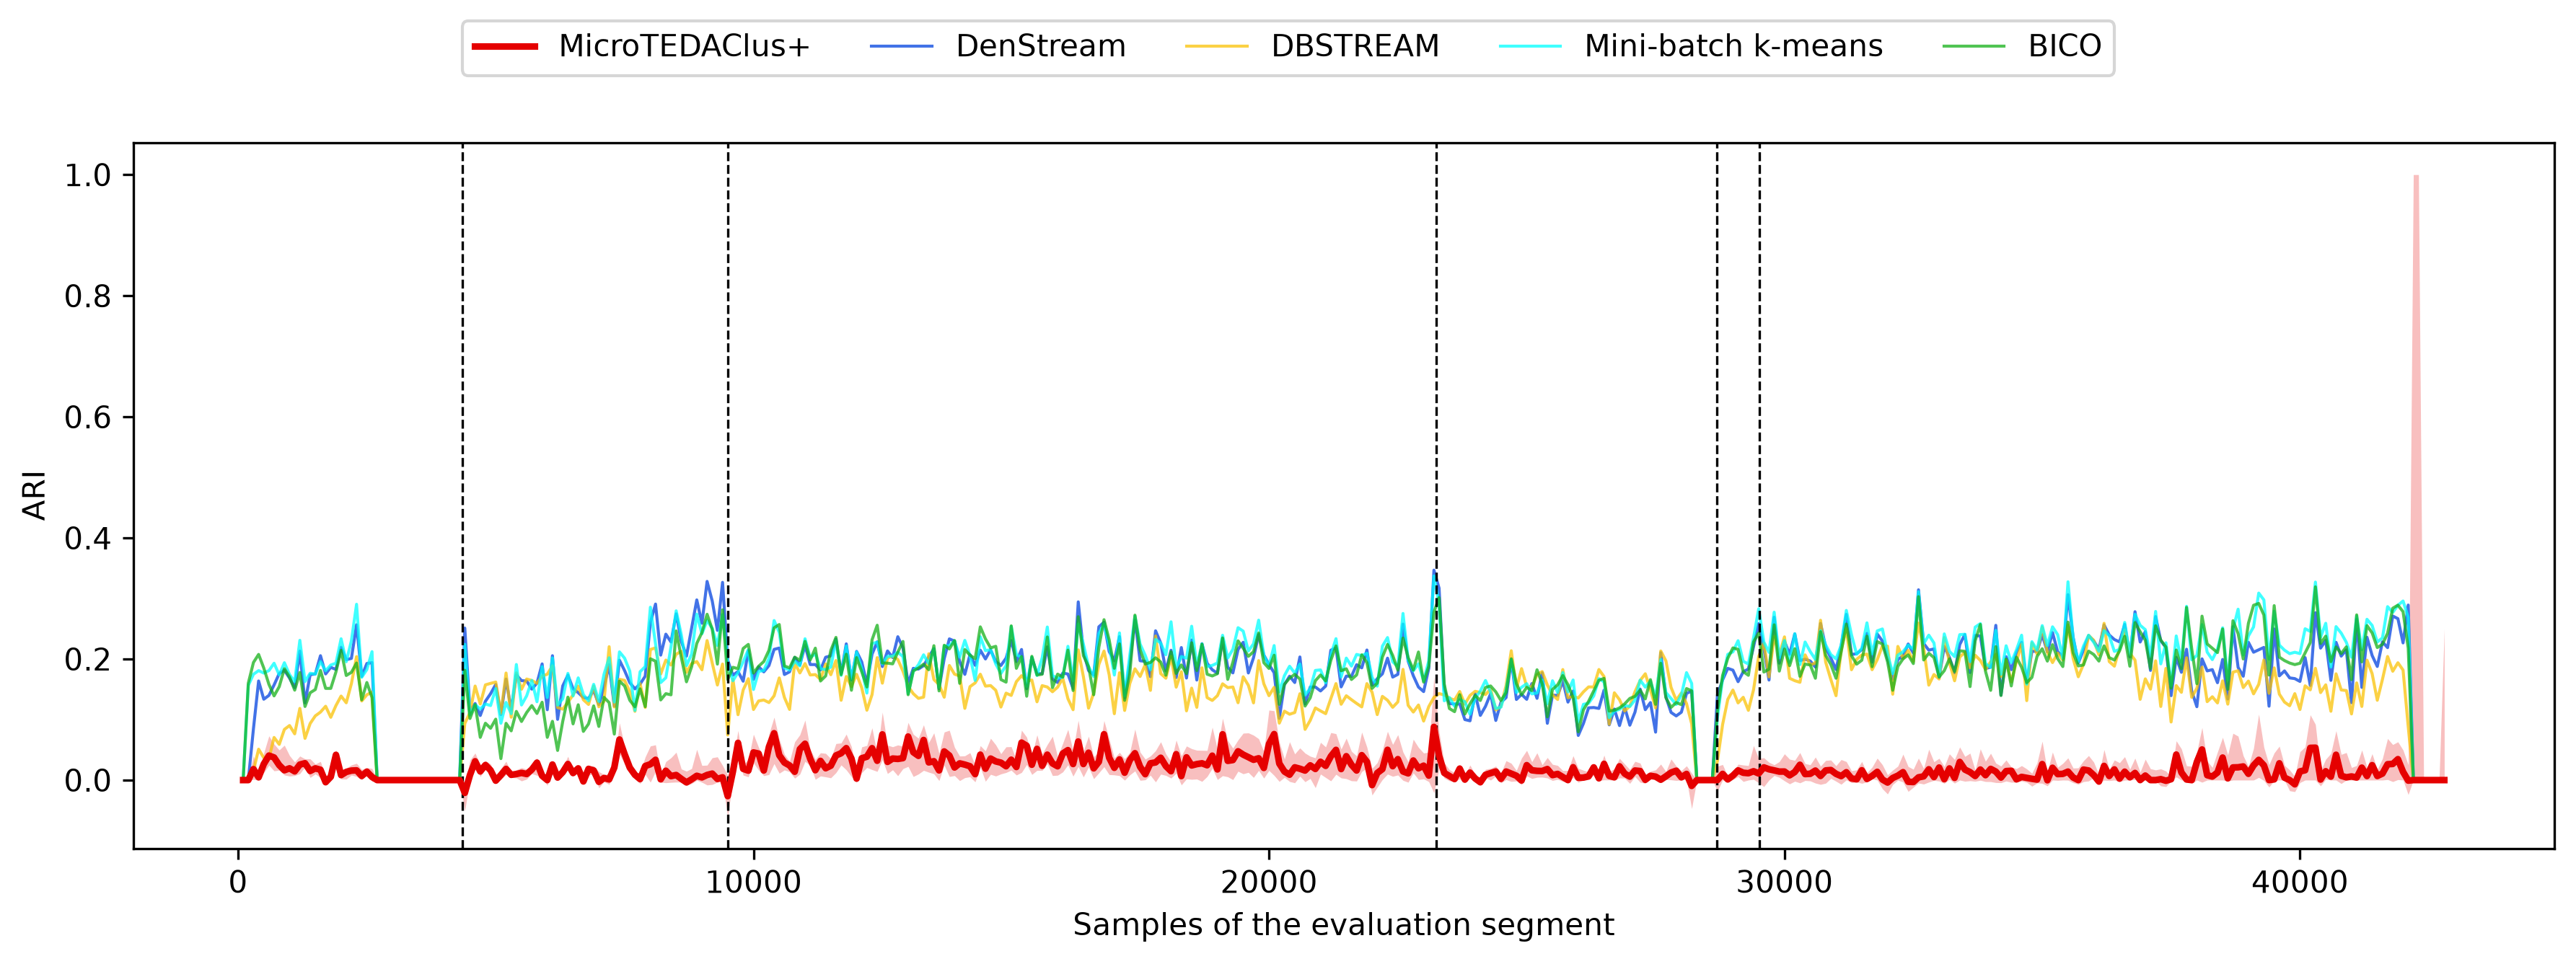
\includegraphics[width=\textwidth]{RealData/artifacts/plots/insects_abrupt.png}
    \caption[Batch ARI along the evaluation segment of \InsectsAbrupt]{Batch ARI of \MicroTEDAClusPlus and the benchmark models along the evaluation segment of \InsectsAbrupt, with the change points of the stream as dashed lines. Medians, with the interquartile band of \MicroTEDAClusPlus, over the 78 runs that every model finished.}
    \label{fig:real_insects_abrupt}
\end{figure}

\Cref{fig:real_insects_abrupt} follows the models along \InsectsAbrupt. \MicroTEDAClusPlus is neither consistently above nor below the benchmark models: it falls below all of them for a stretch after the first change point and rises above all of them for a stretch before the third. In three stretches the median ARI of every model is zero. They are batches of a single class (\cref{tab:real_single_class}), whose ARI is one for a model that placed the whole batch in one cluster and zero otherwise (\cref{subsec:real_order}).

\subsection{Cost}
\label{subsec:real_cost}

\begin{table}[htbp]
\centering
\small
\caption[Execution time and memory of \modelname{MicroTEDAClus+} and the benchmark models on the real datasets]{Execution time and memory of \modelname{MicroTEDAClus+} and the benchmark models on the real datasets: medians over 32 runs, except 28 in INS-A, 25 in INS-I, 26 in INS-R, 22 in GAS, 31 in KDD, 25 in PEN. A dash marks a model left out of a dataset, and every model of a dataset that leaves \MicroTEDAClusPlus{} out.}
\adjustbox{max width=\textwidth, max totalheight=0.82\textheight}{%
\begin{tabular}{l c c c c c c c c }
\toprule
Model & INS-A & INS-I & INS-R & GAS & KDD & COV & PEN & SHU \\
\midrule
\multicolumn{9}{l}{\textit{Learning time [ms]}} \\
\modelname{MicroTEDAClus+} & 5005 & 460 & 8780 & 225 & 2020 & - & 170 & 620 \\
Better/same/worse & 0/1/4 & 3/0/2 & 0/2/3 & 2/2/1 & 3/1/1 & - & 1/1/3 & 0/2/3 \\
\modelname{DenStream} & \textcolor{red}{770} & \textbf{890} & \textcolor{red}{1200} & \textbf{860} & \textbf{7240} & - & \textcolor{red}{90} & \textcolor{red}{220} \\
\modelname{DBSTREAM} & 3630 & \textbf{8770} & 6515 & \textbf{1210} & \textbf{38730} & - & \textbf{520} & 800 \\
\modelname{BIRCH} & \textcolor{red}{1325} & \textbf{1680} & 6715 & 410 & \textbf{12180} & - & 190 & 635 \\
\modelname{Mini-batch k-means} & \textcolor{red}{170} & \textcolor{red}{190} & \textcolor{red}{280} & \textcolor{red}{50} & 1910 & - & \textcolor{red}{30} & \textcolor{red}{185} \\
\modelname{BICO} & \textcolor{red}{130} & \textcolor{red}{150} & \textcolor{red}{210} & 270 & \textcolor{red}{1360} & - & \textcolor{red}{10} & \textcolor{red}{45} \\
\midrule
\multicolumn{9}{l}{\textit{Prediction time [ms]}} \\
\modelname{MicroTEDAClus+} & 65 & 30 & 130 & 20 & 270 & - & 10 & 40 \\
Better/same/worse & 4/1/0 & 5/0/0 & 4/1/0 & 4/1/0 & 5/0/0 & - & 4/1/0 & 5/0/0 \\
\modelname{DenStream} & \textbf{290} & \textbf{370} & \textbf{430} & \textbf{310} & \textbf{3070} & - & \textbf{70} & \textbf{70} \\
\modelname{DBSTREAM} & \textbf{665} & \textbf{310} & \textbf{1195} & \textbf{235} & \textbf{3270} & - & \textbf{110} & \textbf{120} \\
\modelname{BIRCH} & \textbf{230} & \textbf{260} & \textbf{545} & \textbf{75} & \textbf{2320} & - & \textbf{40} & \textbf{190} \\
\modelname{Mini-batch k-means} & 70 & \textbf{80} & 120 & 20 & \textbf{800} & - & 10 & \textbf{80} \\
\modelname{BICO} & \textbf{815} & \textbf{890} & \textbf{1040} & \textbf{240} & \textbf{7160} & - & \textbf{170} & \textbf{490} \\
\midrule
\multicolumn{9}{l}{\textit{Memory held at the end of the stream [KiB]}} \\
\modelname{MicroTEDAClus+} & 396 & 124 & 374 & 461 & 57 & - & 90 & 44 \\
Better/same/worse & 1/2/2 & 3/0/2 & 1/1/3 & 2/1/2 & 3/1/1 & - & 3/0/2 & 1/1/3 \\
\modelname{DenStream} & \textcolor{red}{65} & \textcolor{red}{88} & \textcolor{red}{49} & \textcolor{red}{262} & 62 & - & \textcolor{red}{57} & \textcolor{red}{7} \\
\modelname{DBSTREAM} & 256 & \textbf{722} & \textcolor{red}{224} & 378 & \textbf{295} & - & \textbf{219} & \textcolor{red}{20} \\
\modelname{BIRCH} & \textbf{600} & \textbf{829} & \textbf{1652} & \textbf{2058} & \textbf{475} & - & \textbf{146} & 58 \\
\modelname{Mini-batch k-means} & \textcolor{red}{8} & \textcolor{red}{8} & \textcolor{red}{8} & \textcolor{red}{26} & \textcolor{red}{7} & - & \textcolor{red}{9} & \textcolor{red}{6} \\
\modelname{BICO} & 612 & \textbf{592} & 224 & \textbf{946} & \textbf{412} & - & \textbf{155} & \textbf{94} \\
\midrule
\multicolumn{9}{l}{\textit{Peak memory [KiB]}} \\
\modelname{MicroTEDAClus+} & 12496 & 582 & 14556 & 928 & 231 & - & 1471 & 1562 \\
Better/same/worse & 0/0/5 & 1/3/1 & 0/1/4 & 2/2/1 & 4/0/1 & - & 0/0/5 & 0/0/5 \\
\modelname{DenStream} & \textcolor{red}{528} & 1450 & \textcolor{red}{834} & \textbf{4858} & \textbf{381} & - & \textcolor{red}{366} & \textcolor{red}{134} \\
\modelname{DBSTREAM} & \textcolor{red}{526} & 1016 & \textcolor{red}{472} & 1322 & \textbf{534} & - & \textcolor{red}{344} & \textcolor{red}{92} \\
\modelname{BIRCH} & \textcolor{red}{1774} & \textbf{2949} & 10368 & \textbf{3590} & \textbf{992} & - & \textcolor{red}{305} & \textcolor{red}{132} \\
\modelname{Mini-batch k-means} & \textcolor{red}{34} & \textcolor{red}{33} & \textcolor{red}{30} & \textcolor{red}{85} & \textcolor{red}{22} & - & \textcolor{red}{46} & \textcolor{red}{26} \\
\modelname{BICO} & \textcolor{red}{1208} & 1129 & \textcolor{red}{475} & 1714 & \textbf{612} & - & \textcolor{red}{301} & \textcolor{red}{226} \\
\bottomrule
\end{tabular}
}
\label{tab:real_cost}
\end{table}


\MicroTEDAClusPlus is faster than every benchmark model in the prediction stage of every dataset compared, or indistinguishable from one of them (\cref{tab:real_cost}). In the learning stage it is slower than \MiniBatchKMeans and \BICO in five of the seven datasets compared and than one of the two in the others, and faster than \DBSTREAM in four. The memory it holds at the end of the stream is smaller than that of some benchmark models and larger than that of others, and always larger than that of \MiniBatchKMeans. Its peak during the evaluation is the largest of all models in \InsectsAbrupt, \Pendigits and \Shuttle, and of all but \BIRCH in \InsectsReoccurring.

\section{Summary}
\label{sec:real_summary}

The real datasets add drifts that come from the conditions of the recording, classes that are not drawn from chosen distributions, and up to 128 dimensions. Evaluating on them required standardizing the features by the tuning segment, an order for each stream, search ranges widened and checked by a pilot, \MicroTEDAClusPlus without its noise label, and a limit on the tuning segment and on the size of the summaries. On them, \MicroTEDAClusPlus is better than every benchmark model in \Shuttle, worse than most of them in four datasets, and left out of \Covertype, where its summary exceeds the limit in most runs (\cref{tab:real_quality,tab:real_failures}). It predicts faster than the benchmark models, learns more slowly than the fastest of them, and reaches the largest peak of memory in three datasets (\cref{tab:real_cost}).

\chapter{Model Improvement on Real Data}
\label{chap:real_improvement}

\MicroTEDAClusPlus is indistinguishable from the worst model in six of the eight real datasets of \cref{chap:real_data}, \cref{tab:real_quality}. In this chapter, we repeat on these datasets the effort of \cref{chap:ModelImprovement}: we examine what the model does on them, evaluate changes to it, keep three, and confirm them on new runs and on datasets that took no part in their choice. The result is the final version of \MicroTEDAClusPlus, which we then compare with the benchmark models by the protocol of \cref{chap:real_data}, in quality and in cost. Where the two versions appear together, we call the model of \cref{chap:ModelImprovement} ``\MicroTEDAClusPlus of \cref{chap:ModelImprovement}'', and \modelname{MicroTEDAClus+ (Ch.~\ref{chap:ModelImprovement})} in the tables.

We diagnose the model and develop the changes on six of the eight real datasets, and leave \KDDCup and \Covertype out of both: they are the two longest streams, \cref{tab:real_datasets}, too costly for the many evaluations of the development, and in \Covertype the best model scores lower than in any other dataset, \cref{tab:real_quality}, which leaves little to separate the candidates. The two return in the confirmation, where they show whether the changes hold on data that took no part in their choice.

\section{Diagnosis}
\label{sec:ri_diagnosis}

\begin{table}[htbp]
\centering
\small
\caption[\modelname{MicroTEDAClus+ (Ch.~\ref{chap:ModelImprovement})} on the real datasets of the development]{\modelname{MicroTEDAClus+ (Ch.~\ref{chap:ModelImprovement})} on the real datasets of the development, in the runs of the real-data experiment: medians over the batches of the evaluation segment, then medians over 32 runs, except 31 in GAS. A mature microcluster has three samples or more.}
\adjustbox{max width=\textwidth, max totalheight=0.82\textheight}{%
\begin{tabular}{l c c c c c c }
\toprule
 & INS-A & INS-I & INS-R & GAS & PEN & SHU \\
\midrule
\multicolumn{7}{l}{\textit{Per batch}} \\
Share of the samples labelled as noise & 0.45 & 0.10 & 0.15 & 0.03 & 0.10 & 0.02 \\
Predicted clusters & 3.0 & 7.0 & 1.0 & 9.0 & 8.0 & 8.5 \\
Classes & 5.0 & 6.0 & 5.0 & 6.0 & 10.0 & 3.0 \\
Microclusters & 96.0 & 97.5 & 73.5 & 95.0 & 77.5 & 250.8 \\
Mature microclusters & 12.0 & 9.0 & 8.0 & 53.0 & 15.5 & 187.5 \\
Active microclusters & 11.0 & 8.2 & 4.0 & 28.0 & 12.0 & 83.8 \\
\bottomrule
\end{tabular}
}
\label{tab:ri_diagnosis}
\end{table}


\Cref{tab:ri_diagnosis} gives the state of \cref{chap:ModelImprovement}'s implementation \MicroTEDAClusPlus at every batch of the evaluation segments of the runs of \cref{chap:real_data}, on the six datasets of the development. In the INSECTS datasets and in \Pendigits, most of its microclusters never reach three samples, so few of them mature and fewer are active: the activation, the macroclusters and the prediction rest on a small share of the microclusters. In \GasDrift and \Shuttle, most microclusters mature. In \InsectsAbrupt the model labels nearly half of the samples as noise, and in \InsectsAbrupt and \InsectsReoccurring it predicts fewer clusters than there are classes, a single one in \InsectsReoccurring.

\section{Experimental Design}
\label{sec:ri_design}

The design is that of \cref{sec:mi_design}, with the changes that this section describes. We tune and evaluate every candidate by the protocol of \cref{sec:real_protocol}.

\subsection{Runs}
\label{subsec:ri_runs}

The runs of \cref{chap:real_data} are the runs 0 to 31. We develop the changes on the 32 runs that follow them, and every candidate uses, in each task, the seeds of the previous \MicroTEDAClusPlus version in that task, so that two candidates differ only by their changes. We confirm the kept changes on the runs 0 to 31 of the eight datasets, on which no candidate ran during the development. The INSECTS datasets and \Covertype keep the order of their files, \cref{subsec:real_order}, so every run of them processes the same stream, and their runs differ only in the seeds of the search.

\subsection{Decision Rule}
\label{subsec:ri_decision_rule}

We compare a candidate with its control as in \cref{subsec:mi_decision_rule}, on the Overall ARI of the six datasets and on the Steady-State ARI of the four whose penultimate batch does not hold a single class, \cref{tab:real_single_class}. Unlike in \cref{chap:ModelImprovement}, a candidate does not need to improve its control to be kept. We keep a candidate if

\begin{itemize}
    \item it improves its control;
    \item it is indistinguishable from its control, its change is analytically preferred, and its summary is not clearly larger;
    \item it is mixed, its gains outnumber its losses, and none of its losses, which we examine before the decision, comes from a defect of the change.
\end{itemize}

A kept candidate becomes the control of the candidates that follow it. As the cost of a candidate we report the size of its summary; we did not measure time in the development, since its tasks ran in parallel.

\section{Kept Changes}
\label{sec:ri_kept}

We keep three changes, each applied to the model that results from the previous ones. \Cref{tab:ri_chain} compares every step of the chain with the step before it.

\begin{table}[htbp]
\centering
\caption{The kept changes, each applied to the step above it, on the development runs: medians over the 32 runs less the failed ones. Each row is compared with the row above it over the runs that both finished: a value in bold is significantly better than that of the row above it, and a value in red significantly worse; a smaller summary is better. A dash marks the Steady-State ARI of the streams whose penultimate batch holds a single class. Every failure is a summary that exceeded a quarter of the tuning segment.}
\adjustbox{width=\textwidth, totalheight=0.82\textheight, keepaspectratio}{%
\begin{tabular}{l c c c c c c }
\toprule
Model & INS-A & INS-I & INS-R & GAS & PEN & SHU \\
\midrule
\multicolumn{7}{l}{\textit{Overall ARI}} \\
\modelname{MicroTEDAClus+ (Ch.~\ref{chap:ModelImprovement})} & 0.011 & 0.087 & 0.013 & 0.163 & 0.410 & 0.458 \\
\modelname{low-variance} & \textbf{0.142} & \textbf{0.137} & \textbf{0.107} & 0.154 & \textbf{0.505} & 0.417 \\
\modelname{low-variance + no-noise} & 0.153 & 0.137 & \textbf{0.144} & 0.174 & 0.492 & 0.404 \\
\modelname{low-variance + no-noise + link-factor} & 0.140 & \textcolor{red}{0.111} & \textcolor{red}{0.110} & \textbf{0.203} & \textbf{0.577} & 0.469 \\
\midrule
\multicolumn{7}{l}{\textit{Steady-State ARI}} \\
\modelname{MicroTEDAClus+ (Ch.~\ref{chap:ModelImprovement})} & - & 0.104 & - & 0.093 & 0.377 & 0.415 \\
\modelname{low-variance} & - & 0.164 & - & 0.076 & \textbf{0.543} & 0.365 \\
\modelname{low-variance + no-noise} & - & 0.168 & - & 0.100 & 0.512 & 0.308 \\
\modelname{low-variance + no-noise + link-factor} & - & 0.160 & - & \textbf{0.135} & 0.558 & 0.437 \\
\midrule
\multicolumn{7}{l}{\textit{Steady-state summary}} \\
\modelname{MicroTEDAClus+ (Ch.~\ref{chap:ModelImprovement})} & 78 & 93 & 9 & 112 & 71 & 193 \\
\modelname{low-variance} & \textcolor{red}{451} & \textcolor{red}{106} & \textcolor{red}{215} & 122 & \textcolor{red}{263} & 161 \\
\modelname{low-variance + no-noise} & 671 & 107 & \textcolor{red}{709} & 122 & 259 & 129 \\
\modelname{low-variance + no-noise + link-factor} & 964 & 294 & \textbf{309} & 128 & 286 & \textcolor{red}{383} \\
\midrule
\multicolumn{7}{l}{\textit{Failed runs}} \\
\modelname{MicroTEDAClus+ (Ch.~\ref{chap:ModelImprovement})} & 0 & 0 & 0 & 0 & 0 & 0 \\
\modelname{low-variance} & 1 & 1 & 0 & 0 & 1 & 0 \\
\modelname{low-variance + no-noise} & 4 & 1 & 0 & 0 & 4 & 0 \\
\modelname{low-variance + no-noise + link-factor} & 1 & 0 & 0 & 0 & 2 & 1 \\
\bottomrule
\end{tabular}
}
\label{tab:ri_chain}
\end{table}


\subsection{Variance Limit}
\label{subsec:ri_low_variance}

\modelname{low-variance} searches the variance limit from a tenth of the lower end of the range of the relative variance, \cref{tab:real_rules}. With the range of \cref{chap:real_data}, the selected limit lies at the lower end of its range in most runs of \InsectsAbrupt, \InsectsIncremental and \Pendigits, \cref{tab:ri_variance}, so the search would select smaller limits if it could. With the extended range, it lies at the lower end in no run.

\begin{table}[htbp]
\centering
\caption{Percentage of the development runs in which the selected variance limit lies within a twentieth of the width of its range from its lower end, in the logarithmic scale of the search.}
\adjustbox{width=\textwidth, totalheight=0.82\textheight, keepaspectratio}{%
\begin{tabular}{l c c c c c c }
\toprule
Model & INS-A & INS-I & INS-R & GAS & PEN & SHU \\
\midrule
\multicolumn{7}{l}{\textit{Variance limit at the lower end of its range}} \\
\modelname{MicroTEDAClus+ (Ch.~3)} & 75 & 84 & 34 & 0 & 81 & 0 \\
\modelname{low-variance} & 0 & 0 & 0 & 0 & 0 & 0 \\
\bottomrule
\end{tabular}
}
\label{tab:ri_variance}
\end{table}


The change widens the search of \MicroTEDAClusPlus and of no other model. The ranges of \cref{chap:real_data} come from the tuning segment by rule, so a wider range does not suit one scale only. In that chapter, we extended the lower end of the distances of the benchmark models to a tenth of the median distance from a sample to its nearest neighbour, \cref{tab:real_rules}, and left the lower end of the relative variance at the square of that distance.

\modelname{low-variance} improves \MicroTEDAClusPlus of \cref{chap:ModelImprovement} in the Overall ARI of the three INSECTS datasets and of \Pendigits, and in the Steady-State ARI of \Pendigits, \cref{tab:ri_chain}. Its steady-state summary is larger where it improves.

\subsection{Noise Label}
\label{subsec:ri_no_noise}

\modelname{no-noise} removes the noise label of \MicroTEDAClusPlus, \cref{eq:mi_final_prediction}: the model assigns every sample to the macrocluster of its nearest active microcluster, and the noise distance is no longer a hyperparameter. The classes of the real datasets cover every sample, \cref{sec:real_datasets}, so a sample labelled as noise is always an error of the partition, and the previous version of \MicroTEDAClusPlus labels nearly half of the samples of \InsectsAbrupt as noise, \cref{tab:ri_diagnosis}.

\modelname{low-variance + no-noise} improves \modelname{low-variance} in the Overall ARI of \InsectsReoccurring, and loses in no dataset, \cref{tab:ri_chain}. It fails in more runs, and its summary is larger in \InsectsReoccurring.

\subsection{Link Factor}
\label{subsec:ri_link}

\modelname{link-factor} is the candidate of \cref{subsec:mi_improvement_candidates} that searches the factor $\ell$ of the intersection condition, \cref{eq:microcluster_intersection_condition}, in $[0.5, 4]$. Applied to \modelname{low-variance}, it improves it with a single gain, while its median Overall ARI is lower in four of the six datasets, \cref{tab:ri_candidates}. Since we kept \modelname{no-noise} against the same control, we evaluate the two changes together: we keep \modelname{link-factor} if we keep \modelname{low-variance + no-noise + link-factor} against \modelname{low-variance + no-noise}.

The combination is mixed, \cref{tab:ri_chain}: it gains in the Overall ARI of \GasDrift and \Pendigits and in the Steady-State ARI of \GasDrift, and loses in the Overall ARI of \InsectsIncremental and \InsectsReoccurring. The search selects factors close to the fixed factor of two in the INSECTS datasets and different factors in the others, \cref{tab:ri_link}.

\begin{table}[htbp]
\centering
\caption{Link factor selected on the development runs: median and quartile coefficient of dispersion.}
\adjustbox{width=\textwidth, totalheight=0.82\textheight, keepaspectratio}{%
\begin{tabular}{l c c c c c c }
\toprule
 & INS-A & INS-I & INS-R & GAS & PEN & SHU \\
\midrule
\multicolumn{7}{l}{\textit{\modelname{low-variance + no-noise + link-factor}}} \\
Link factor & 2.40 [0.20] & 2.14 [0.20] & 2.04 [0.21] & 2.84 [0.17] & 1.17 [0.09] & 3.41 [0.15] \\
\bottomrule
\end{tabular}
}
\label{tab:ri_link}
\end{table}


Where the selected factor is that of the control, the model is nearly the control, found by a search with one more hyperparameter and the same number of trials, which we already found to cost quality in \cref{subsec:mi_m_function}. We attribute the losses to the search and not to the change, and the gains outnumber them, so we keep the combination.

\section{Rejected Candidates}
\label{sec:ri_rejected}

\Cref{tab:ri_candidates} gives the outcome of every other candidate against its control. Its last rows are \modelname{link-factor} applied alone to \modelname{low-variance}, before the combination test of \cref{subsec:ri_link}, and \modelname{wide-link} against its control and against the last step of the chain.

\begin{table}[htbp]
\centering
\small
\caption[The candidates outside the chain of kept changes]{The candidates outside the chain of kept changes, each against its control on the development runs: outcome of the decision rule, significant gains and losses, datasets where its median Overall ARI is lower, and datasets where its steady-state summary is significantly larger or smaller. The covariance was evaluated on eight runs of three datasets.}
\adjustbox{max width=\textwidth, max totalheight=0.82\textheight}{%
\begin{tabular}{l l c c c c c c}
\toprule
Candidate & Control & Outcome & Gains & Losses & Lower & Larger & Smaller \\
\midrule
\variant{m-fixed} & \variant{low-variance} & regresses & 0 & 7 & 6 & 0 & 6 \\
\variant{m-constant} & \variant{low-variance} & regresses & 0 & 7 & 6 & 0 & 6 \\
\variant{m-sigmoid} & \variant{low-variance} & regresses & 0 & 5 & 5 & 0 & 0 \\
\variant{m-reparam} & \variant{low-variance} & regresses & 0 & 2 & 3 & 0 & 0 \\
\variant{m-rate} & \variant{low-variance} & regresses & 0 & 2 & 5 & 0 & 0 \\
\variant{chi-threshold} & \variant{low-variance} & improves & 1 & 0 & 5 & 0 & 0 \\
\variant{diagonal-variance} & \variant{low-variance} & regresses & 0 & 5 & 5 & 0 & 2 \\
\variant{covariance} & \variant{low-variance} & regresses & 0 & 2 & 2 & 0 & 1 \\
\variant{volume-density} & \variant{low-variance} & mixed & 1 & 1 & 4 & 1 & 0 \\
\variant{log-density} & \variant{low-variance} & regresses & 0 & 6 & 6 & 0 & 2 \\
\variant{diagonal-variance + log-density} & \variant{low-variance} & not run & - & - & - & - & - \\
\variant{no-activation} & \variant{low-variance} & mixed & 2 & 6 & 5 & 4 & 0 \\
\variant{mature-mean} & \variant{low-variance} & indistinguishable & 0 & 0 & 4 & 1 & 0 \\
\variant{recency} & \variant{low-variance} & mixed & 2 & 3 & 5 & 2 & 0 \\
\variant{dimensionality-penalty} & \variant{low-variance} & mixed & 2 & 4 & 5 & 0 & 6 \\
\variant{norm-typicality} & \variant{low-variance} & regresses & 0 & 10 & 6 & 0 & 2 \\
\variant{local-weights} & \variant{low-variance} & regresses & 0 & 9 & 6 & 0 & 0 \\
\variant{link-factor} & \variant{low-variance} & improves & 1 & 0 & 4 & 1 & 1 \\
\variant{wide-link} & \variant{low-variance + no-noise} & mixed & 1 & 1 & 3 & 1 & 3 \\
\variant{wide-link} & \variant{low-variance + no-noise + link-factor} & improves & 2 & 0 & 5 & 0 & 3 \\
\bottomrule
\end{tabular}
}
\label{tab:ri_candidates}
\end{table}


\paragraph{Sensitivity function.} \modelname{m-constant} and \modelname{m-reparam} are the candidates of \cref{subsec:mi_m_function}, and three more change the function $m$ of \cref{eq:m_function}: \modelname{m-fixed} sets $m = 3$ from the third sample on, \modelname{m-sigmoid} searches the two constants of the sigmoid, and \modelname{m-rate} keeps the asymptote of three and searches how fast $m$ approaches it. All five regress, and we retain the original function, as in \cref{chap:ModelImprovement}.

\paragraph{Geometry.} \modelname{diagonal-variance} gives a microcluster one variance per feature, and \modelname{covariance} is the candidate of \cref{subsec:mi_covariance} with the directional link. Both regress. We evaluated \modelname{covariance} first on eight runs of \InsectsIncremental, \Pendigits and \Shuttle, three datasets with fewer features than \GasDrift, because each of its microclusters carries a matrix of the square of the dimension and a full development would have taken several hours, most of them in \GasDrift. Its probe already lost in two cells, and \modelname{diagonal-variance}, which also standardizes the distance feature by feature, had regressed in five, so we did not run the full development. We retain the scalar variance.

\paragraph{Density.} \modelname{volume-density} is the density of \cref{sec:mi_corrections}, and \modelname{log-density} is the logarithm of the number of samples per volume of the microcluster. \modelname{volume-density} is mixed with one gain and one loss, which the rule does not keep, and \modelname{log-density} regresses. We did not run \modelname{diagonal-variance + log-density}, since both of its changes regress alone and the pair would have to undo both regressions to be kept.

\paragraph{Activation and pruning.} Two candidates of \cref{subsec:mi_improvement_candidates}, \modelname{no-activation} and \modelname{recency}, are mixed, with more losses than gains. \modelname{mature-mean}, the correction of \cref{sec:mi_corrections}, is indistinguishable from its control and analytically preferred, but its summary is larger in one dataset, so we do not keep it.

\paragraph{Membership.} \modelname{norm-typicality} and \modelname{local-weights} are the memberships of \cref{sec:mi_corrections}. Both regress, and we retain the nearest membership.

\paragraph{Dimensionality penalty.} \modelname{dimensionality-penalty} restores the factor $2/d$ that we removed from \MicroTEDAClusPlus in \cref{chap:ModelImprovement}. It is mixed, with more losses than gains, and its summary is smaller than that of its control in every dataset.

\paragraph{Departures from the rule.} We did not keep two candidates that the rule would keep. \modelname{chi-threshold}, the candidate of \cref{subsec:mi_improvement_candidates} that tests the outliers against the dispersion of a Gaussian cluster in $d$ dimensions, improves \modelname{low-variance} with a single gain, \cref{tab:ri_candidates}, while its median Overall ARI is lower in five of the six datasets. \modelname{wide-link}, the link factor searched in $[0.05, 4]$ on a logarithmic scale, is mixed against its control, \modelname{low-variance + no-noise}, with one gain and one loss, but in the direct comparison planned between it and \modelname{low-variance + no-noise + link-factor} it improves the latter with two gains, while its median Overall ARI is lower in five of the six datasets. In both cases we judged a single favourable dataset to weigh less than a consistent lean in the others, and kept the model without the candidate. We also compared the medians of the two link factors with those of the benchmark models in \cref{tab:real_quality}, outside the rule, and that comparison favoured the narrower range. We kept the link factor itself only provisionally, although it improved its control, because its median Overall ARI was also lower in most datasets; what distinguished it from \modelname{chi-threshold} was the size of its gain, which the rule does not consider. The combination test of \cref{subsec:ri_link} then kept it by the rule. Finally, we did not evaluate \modelname{covariance} and \modelname{diagonal-variance + log-density} in full, for the reasons given with them above.

\section{Confirmation}
\label{sec:ri_confirmation}

\begin{table}[htbp]
\centering
\small
\caption[The kept changes, each applied to the step above it, on the runs of the real-data experiment]{The kept changes, each applied to the step above it, on the runs of the real-data experiment: medians over the 32 runs less the failed ones, each row compared with the row above it over the runs that both finished. A dash marks the Steady-State ARI of a stream whose penultimate batch holds a single class; every failure is a summary over its limit.}
\adjustbox{max width=\textwidth, max totalheight=0.82\textheight}{%
\begin{tabular}{l c c c c c c c c }
\toprule
Model & INS-A & INS-I & INS-R & GAS & KDD & COV & PEN & SHU \\
\midrule
\multicolumn{9}{l}{\textit{Overall ARI}} \\
\modelname{MicroTEDAClus+ (Ch.~\ref{chap:ModelImprovement})} & 0.017 & 0.088 & 0.012 & 0.162 & 0.669 & 0.000 & 0.414 & 0.444 \\
\variant{low-variance} & \textbf{0.138} & \textbf{0.116} & \textbf{0.124} & 0.164 & 0.671 & 0.000 & \textbf{0.530} & 0.433 \\
\variant{low-variance + no-noise} & 0.152 & 0.133 & \textbf{0.144} & 0.170 & 0.697 & 0.052 & 0.500 & 0.468 \\
\variant{low-variance + no-noise + link-factor} & 0.142 & 0.128 & \textcolor{red}{0.106} & 0.192 & 0.689 & \textbf{0.059} & \textbf{0.581} & 0.500 \\
\midrule
\multicolumn{9}{l}{\textit{Steady-State ARI}} \\
\modelname{MicroTEDAClus+ (Ch.~\ref{chap:ModelImprovement})} & - & 0.103 & - & 0.097 & 0.644 & - & 0.356 & 0.399 \\
\variant{low-variance} & - & 0.161 & - & 0.092 & 0.657 & - & \textbf{0.541} & 0.405 \\
\variant{low-variance + no-noise} & - & 0.164 & - & 0.129 & 0.665 & - & 0.515 & 0.422 \\
\variant{low-variance + no-noise + link-factor} & - & 0.153 & - & 0.142 & 0.637 & - & 0.576 & 0.460 \\
\midrule
\multicolumn{9}{l}{\textit{Steady-state summary}} \\
\modelname{MicroTEDAClus+ (Ch.~\ref{chap:ModelImprovement})} & 81 & 94 & 9 & 100 & 12 & 4 & 74 & 182 \\
\variant{low-variance} & \textcolor{red}{326} & \textcolor{red}{102} & \textcolor{red}{748} & 117 & 12 & 5 & \textcolor{red}{370} & 136 \\
\variant{low-variance + no-noise} & 1018 & 108 & 773 & 112 & 16 & 2138 & 262 & 182 \\
\variant{low-variance + no-noise + link-factor} & 1002 & 304 & \textbf{376} & 83 & 17 & 722 & 226 & 329 \\
\midrule
\multicolumn{9}{l}{\textit{Failed runs}} \\
\modelname{MicroTEDAClus+ (Ch.~\ref{chap:ModelImprovement})} & 0 & 0 & 0 & 1 & 0 & 0 & 0 & 0 \\
\variant{low-variance} & 2 & 0 & 0 & 0 & 0 & 14 & 3 & 0 \\
\variant{low-variance + no-noise} & 2 & 0 & 0 & 0 & 0 & 17 & 3 & 0 \\
\variant{low-variance + no-noise + link-factor} & 0 & 0 & 2 & 0 & 0 & 8 & 1 & 1 \\
\bottomrule
\end{tabular}
}
\label{tab:ri_confirmation}
\end{table}


\Cref{tab:ri_confirmation} repeats the chain on the runs 0 to 31 of the eight datasets. \modelname{low-variance} improves the previous \MicroTEDAClusPlus version in the Overall ARI of the three INSECTS datasets and of \Pendigits and in the Steady-State ARI of \Pendigits, the same gains as in the development, \cref{tab:ri_chain}, and its summary is again larger where it improves. The removal of the noise label improves \modelname{low-variance} in \InsectsReoccurring, as in the development. The link factor gains in \Pendigits and loses in \InsectsReoccurring, as in the development, and also gains in \Covertype; its gain in \GasDrift and its loss in \InsectsIncremental are not significant on these runs.

No step loses where the development found it to gain, and no step loses in the two datasets that took no part in the development. In \KDDCup no step changes the model significantly. In \Covertype the steps fail in many runs, all by the limit on the summary of \cref{sec:real_protocol}, \cref{tab:ri_confirmation}.

\section{The Final Version of \MicroTEDAClusPlus}
\label{sec:ri_final}

The final version of \MicroTEDAClusPlus differs from the version of \cref{chap:ModelImprovement} in the three points of \cref{tab:ri_differences}. Its hyperparameters are the relative variance limit $r$, the decay and the link factor $\ell$.

\begin{table}[htbp]
\centering
\caption{Differences between the final version of \MicroTEDAClusPlus and the version of \cref{chap:ModelImprovement}.}
\begin{tabular}{l p{0.36\textwidth} p{0.36\textwidth}}
\toprule
 & Version of \cref{chap:ModelImprovement} & Final version \\
\midrule
Noise & a sample farther than $n_\sigma$ standard deviations from every active microcluster is noise & every sample is assigned to the macrocluster of its nearest active microcluster \\
Intersection & $\lVert \mu_i - \mu_j \rVert \le 2\,(\sigma_i + \sigma_j)$ & $\lVert \mu_i - \mu_j \rVert \le \ell\,(\sigma_i + \sigma_j)$, with $\ell$ searched in $[0.5, 4]$ \\
Variance limit & searched from the square of the median distance from a sample to its nearest neighbour, as a fraction of the total variance & searched from a tenth of that lower end \\
\bottomrule
\end{tabular}
\label{tab:ri_differences}
\end{table}

We tune and evaluate the final version by the protocol of \cref{chap:real_data} on its runs 0 to 31, as every model of that chapter, and measure its time and memory, and those of the benchmark models, by the procedure of \cref{sec:mod_measurements} on the runs 0 to 9. Its search uses seeds of its own, as that of every model of \cref{chap:real_data}, where the confirmation used those of \MicroTEDAClusPlus of \cref{chap:ModelImprovement} to pair the steps, so its medians differ somewhat from those of the last step of \cref{tab:ri_confirmation}.

\begin{table}[htbp]
\centering
\caption{The partitions of the two versions of \MicroTEDAClusPlus{} on the real datasets: medians over the batches of the evaluation segment, then medians over the runs, at least 32 runs, except 27 in COV, 31 in GAS, 31 in INS-A, 31 in INS-R, 30 in PEN. Homogeneity and completeness compare the clusters predicted for a batch with its classes, over the samples not labelled as noise.}
\adjustbox{width=\textwidth, totalheight=0.82\textheight, keepaspectratio}{%
\begin{tabular}{l c c c c c c c c }
\toprule
Model & INS-A & INS-I & INS-R & GAS & KDD & COV & PEN & SHU \\
\midrule
\multicolumn{9}{l}{\textit{Clusters per batch}} \\
Classes & 5.0 & 6.0 & 5.0 & 6.0 & 4.0 & 2.0 & 10.0 & 3.0 \\
\modelname{MicroTEDAClus+ (Ch.~3)} & 3.0 & 7.0 & 1.0 & 9.0 & 1.0 & 1.0 & 8.0 & 8.5 \\
\modelname{MicroTEDAClus+} & 27.0 & 14.0 & 13.0 & 9.0 & 2.0 & 19.0 & 18.0 & 6.0 \\
\midrule
\multicolumn{9}{l}{\textit{Share of the samples labelled as noise}} \\
\modelname{MicroTEDAClus+ (Ch.~3)} & 0.45 & 0.10 & 0.15 & 0.03 & 0.44 & 0.00 & 0.10 & 0.02 \\
\modelname{MicroTEDAClus+} & 0.00 & 0.00 & 0.00 & 0.00 & 0.00 & 0.00 & 0.00 & 0.00 \\
\midrule
\multicolumn{9}{l}{\textit{Homogeneity}} \\
\modelname{MicroTEDAClus+ (Ch.~3)} & 0.09 & 0.27 & 0.00 & 0.40 & 1.00 & 0.00 & 0.65 & 0.61 \\
\modelname{MicroTEDAClus+} & 0.60 & 0.42 & 0.42 & 0.38 & 0.59 & 0.71 & 0.83 & 0.57 \\
\midrule
\multicolumn{9}{l}{\textit{Completeness}} \\
\modelname{MicroTEDAClus+ (Ch.~3)} & 0.51 & 0.36 & 1.00 & 0.47 & 1.00 & 1.00 & 0.78 & 0.41 \\
\modelname{MicroTEDAClus+} & 0.32 & 0.35 & 0.30 & 0.41 & 0.86 & 0.16 & 0.71 & 0.48 \\
\bottomrule
\end{tabular}
}
\label{tab:ri_partitions}
\end{table}


\Cref{tab:ri_partitions} compares the partitions that the two versions predict. The final version labels no sample as noise, and in every dataset but \KDDCup it predicts more clusters than there are classes, several times more in \InsectsAbrupt and \Covertype. Its homogeneity is higher than that of the version of \cref{chap:ModelImprovement} in five datasets and its completeness is lower in most: the final version splits the classes over more clusters, where the version of \cref{chap:ModelImprovement} merged them or labelled their samples as noise. Where the version of \cref{chap:ModelImprovement} predicts a single cluster, in \InsectsReoccurring, \KDDCup and \Covertype, its completeness is one by construction.

\section{Comparison with the Benchmark Models}
\label{sec:ri_comparison}

\subsection{Clustering Quality}
\label{subsec:ri_quality}

\begin{table}[htbp]
\centering
\small
\caption[Clustering quality of \modelname{MicroTEDAClus+} and the benchmark models on the real datasets]{Clustering quality of \modelname{MicroTEDAClus+} and the benchmark models on the real datasets: medians over 94 runs, except 90 in INS-A, 93 in INS-I, 59 in INS-R, 93 in GAS, 54 in KDD, 70 in COV, 81 in PEN. A dash marks a value left out: the Steady-State ARI of a stream whose penultimate batch holds a single class, or a model that failed in more than half of the runs of a dataset.}
\adjustbox{max width=\textwidth, max totalheight=0.82\textheight}{%
\begin{tabular}{l c c c c c c c c }
\toprule
Model & INS-A & INS-I & INS-R & GAS & KDD & COV & PEN & SHU \\
\midrule
\multicolumn{9}{l}{\textit{Overall ARI}} \\
\modelname{MicroTEDAClus+} & 0.147 & 0.134 & 0.105 & 0.184 & 0.665 & 0.058 & 0.585 & 0.463 \\
Better/same/worse & 0/2/2 & 1/0/3 & 1/2/2 & 2/1/1 & 1/1/3 & 0/1/4 & 1/4/0 & 5/0/0 \\
\modelname{DenStream} & \textcolor{red}{0.169} & \textcolor{red}{0.174} & \textcolor{red}{0.153} & 0.184 & \textcolor{red}{0.946} & 0.056 & \textbf{0.506} & \textbf{0.390} \\
\modelname{DBSTREAM} & 0.156 & \textbf{0.089} & 0.084 & \textbf{0.151} & \textcolor{red}{0.916} & \textcolor{red}{0.069} & 0.539 & \textbf{0.364} \\
\modelname{BIRCH} & - & - & \textbf{0.062} & - & \textbf{0.066} & \textcolor{red}{0.065} & 0.530 & \textbf{0.000} \\
\modelname{Mini-batch k-means} & 0.173 & \textcolor{red}{0.167} & 0.115 & \textcolor{red}{0.206} & \textcolor{red}{0.909} & \textcolor{red}{0.073} & 0.529 & \textbf{0.428} \\
\modelname{BICO} & \textcolor{red}{0.182} & \textcolor{red}{0.162} & \textcolor{red}{0.124} & \textbf{0.157} & 0.562 & \textcolor{red}{0.069} & 0.544 & \textbf{0.353} \\
\midrule
\multicolumn{9}{l}{\textit{Steady-State ARI}} \\
\modelname{MicroTEDAClus+} & - & 0.165 & - & 0.143 & 0.581 & - & 0.533 & 0.397 \\
Better/same/worse & - & 1/0/3 & - & 1/3/0 & 1/1/3 & - & 0/5/0 & 2/3/0 \\
\modelname{DenStream} & - & \textcolor{red}{0.252} & - & 0.132 & \textcolor{red}{0.941} & - & 0.500 & 0.385 \\
\modelname{DBSTREAM} & - & \textbf{0.108} & - & 0.116 & \textcolor{red}{0.889} & - & 0.501 & 0.326 \\
\modelname{BIRCH} & - & - & - & - & \textbf{0.022} & - & 0.530 & \textbf{0.000} \\
\modelname{Mini-batch k-means} & - & \textcolor{red}{0.222} & - & 0.135 & \textcolor{red}{0.896} & - & 0.532 & 0.378 \\
\modelname{BICO} & - & \textcolor{red}{0.223} & - & \textbf{0.113} & 0.526 & - & 0.551 & \textbf{0.297} \\
\bottomrule
\end{tabular}
}
\label{tab:ri_quality}
\end{table}

\begin{table}[htbp]
\centering
\caption{Number of runs in which \modelname{MicroTEDAClus+} failed on a real dataset. Every failure is a summary that exceeded a quarter of the tuning segment.}
\adjustbox{width=\textwidth, totalheight=0.82\textheight, keepaspectratio}{%
\begin{tabular}{l c c c c c c c c }
\toprule
Model & INS-A & INS-I & INS-R & GAS & KDD & COV & PEN & SHU \\
\midrule
\multicolumn{9}{l}{\textit{Failed runs}} \\
\modelname{MicroTEDAClus+} & 1 & 0 & 1 & 0 & 0 & 5 & 2 & 0 \\
\bottomrule
\end{tabular}
}
\label{tab:ri_failures}
\end{table}


In the Overall ARI, \cref{tab:ri_quality}, the final version of \MicroTEDAClusPlus is indistinguishable from the best model in \Shuttle, where no other model is, and from the worst in \InsectsAbrupt, \GasDrift and \Covertype; in \InsectsAbrupt its median is the lowest of the models compared. In the four other datasets it is in neither group. In the same comparison, \MicroTEDAClusPlus of \cref{chap:ModelImprovement} was indistinguishable from the worst model in six datasets, \cref{tab:real_quality}. In \KDDCup the median of the final version is about that of the version of \cref{chap:ModelImprovement}.

At the penultimate batch, the final version is indistinguishable from the best model in \GasDrift and \Shuttle and from the worst in \InsectsIncremental. At the fifth batch it is indistinguishable from the worst in the three INSECTS datasets and in \KDDCup, so it still starts slowly, and its maximum ARI drop is among the largest in \InsectsIncremental, \Pendigits and \Shuttle. It fails in nine runs, most of them in \Covertype, all by the limit on the summary, \cref{tab:ri_failures}.

\subsection{Cost}
\label{subsec:ri_cost}

\begin{table}[htbp]
\centering
\caption{Execution time and memory of the models on the real datasets, each task measured alone and its memory counted from every allocation of its process: medians over 10 runs, except 9 in INS-A, 6 in INS-R, 4 in KDD, 7 in COV, 9 in PEN. A value in bold is statistically indistinguishable from the best model of its dataset, and a value in red from the worst. A dash marks a model left out of a dataset.}
\adjustbox{width=\textwidth, totalheight=0.82\textheight, keepaspectratio}{%
\begin{tabular}{l c c c c c c c c }
\toprule
Model & INS-A & INS-I & INS-R & GAS & KDD & COV & PEN & SHU \\
\midrule
\multicolumn{9}{l}{\textit{Learning time of the evaluation segment, in milliseconds}} \\
\modelname{MicroTEDAClus+} & \textcolor{red}{2040} & 500 & 3695 & \textcolor{red}{210} & 1970 & 25060 & 50 & \textcolor{red}{1695} \\
\modelname{DenStream} & \textcolor{red}{790} & 1905 & 1165 & \textcolor{red}{785} & 7970 & 3470 & 90 & 220 \\
\modelname{DBSTREAM} & \textcolor{red}{6490} & \textcolor{red}{5670} & 6595 & \textcolor{red}{1115} & 64720 & 26580 & \textcolor{red}{820} & \textcolor{red}{845} \\
\modelname{BIRCH} & - & - & 6510 & - & 12045 & 7470 & 190 & \textcolor{red}{650} \\
\modelname{Mini-batch k-means} & \textbf{170} & 190 & 280 & \textbf{50} & 1910 & 2190 & 30 & 190 \\
\modelname{BICO} & \textbf{120} & \textbf{135} & 200 & 240 & 1215 & 590 & \textbf{10} & \textbf{40} \\
\midrule
\multicolumn{9}{l}{\textit{Prediction time of the evaluation segment, in milliseconds}} \\
\modelname{MicroTEDAClus+} & \textbf{60} & \textbf{30} & 70 & \textbf{10} & 225 & 1290 & \textbf{0} & \textbf{55} \\
\modelname{DenStream} & 300 & 410 & 420 & \textcolor{red}{410} & 2945 & 1460 & 50 & \textbf{70} \\
\modelname{DBSTREAM} & \textcolor{red}{870} & \textcolor{red}{425} & 1505 & \textcolor{red}{335} & 3525 & 5470 & 150 & 145 \\
\modelname{BIRCH} & - & - & 540 & - & 2340 & 2300 & 40 & 190 \\
\modelname{Mini-batch k-means} & \textbf{70} & 80 & 115 & \textbf{20} & 790 & 930 & \textbf{10} & \textbf{80} \\
\modelname{BICO} & \textcolor{red}{710} & \textcolor{red}{770} & 1040 & 255 & 6900 & 8210 & \textcolor{red}{170} & \textcolor{red}{505} \\
\midrule
\multicolumn{9}{l}{\textit{Memory held at the end of the stream, in KiB}} \\
\modelname{MicroTEDAClus+} & \textcolor{red}{191} & 124 & 268 & 449 & 56 & 186 & 34 & \textcolor{red}{92} \\
\modelname{DenStream} & 65 & 101 & 60 & 375 & 58 & 16 & 53 & \textbf{7} \\
\modelname{DBSTREAM} & \textcolor{red}{599} & \textcolor{red}{446} & 252 & \textcolor{red}{304} & 448 & 103 & \textcolor{red}{382} & 22 \\
\modelname{BIRCH} & - & - & 1587 & - & 478 & 44 & \textcolor{red}{169} & \textcolor{red}{44} \\
\modelname{Mini-batch k-means} & \textbf{8} & \textbf{8} & 7 & \textbf{22} & 8 & 8 & \textbf{9} & \textbf{5} \\
\modelname{BICO} & \textcolor{red}{188} & \textcolor{red}{184} & 176 & \textcolor{red}{676} & 331 & 43 & 173 & \textcolor{red}{52} \\
\midrule
\multicolumn{9}{l}{\textit{Peak memory during the evaluation, in KiB}} \\
\modelname{MicroTEDAClus+} & \textcolor{red}{3700} & \textcolor{red}{578} & 4464 & \textcolor{red}{829} & 244 & 12097 & \textcolor{red}{332} & \textcolor{red}{5613} \\
\modelname{DenStream} & \textcolor{red}{630} & \textcolor{red}{2273} & 528 & \textcolor{red}{4474} & 1576 & 142 & \textcolor{red}{364} & 142 \\
\modelname{DBSTREAM} & \textcolor{red}{870} & \textcolor{red}{714} & 480 & 1355 & 700 & 324 & \textcolor{red}{509} & 94 \\
\modelname{BIRCH} & - & - & 10104 & - & 1004 & 97 & \textcolor{red}{377} & 106 \\
\modelname{Mini-batch k-means} & \textbf{34} & \textbf{26} & 24 & \textbf{67} & 22 & 32 & \textbf{45} & \textbf{17} \\
\modelname{BICO} & 397 & \textcolor{red}{420} & 422 & \textcolor{red}{1293} & 554 & 198 & \textcolor{red}{320} & 166 \\
\bottomrule
\end{tabular}
}
\label{tab:ri_cost}
\end{table}


The final version is indistinguishable from the fastest model in the prediction stage in five datasets, and from the slowest in none, \cref{tab:ri_cost}. In the learning stage it is indistinguishable from the slowest in \InsectsAbrupt, \GasDrift and \Shuttle and from the fastest in none; the models indistinguishable from the fastest in that stage are \MiniBatchKMeans and \BICO. The memory it holds at the end of the stream is among the largest in \InsectsAbrupt and \Shuttle, and its peak during the evaluation is among the highest in five datasets. \MiniBatchKMeans holds the least memory in five datasets. These comparisons rest on ten runs, and on fewer where a model failed.

\subsection{Remaining Limits}
\label{subsec:ri_limits}

Three limits of the final version remain. It splits the classes of the INSECTS datasets over many clusters, \cref{tab:ri_partitions}, while its search selects there a link factor close to the fixed factor of the version of \cref{chap:ModelImprovement}, \cref{tab:ri_link}, although a larger factor would join more microclusters. It starts slowly, \cref{tab:ri_quality}. And its summary exceeds the limit in some runs of \Covertype, \cref{tab:ri_failures}, and the peak of its memory is among the highest, \cref{tab:ri_cost}.

We evaluated the final version on the real datasets only, and not on the synthetic datasets of \cref{chap:modernization}. Its removal of the noise label suits data whose classes cover every sample, while on the synthetic datasets with noise we found the noise label to improve the model, \cref{sec:mi_improvements}.

\section{Summary}
\label{sec:ri_summary}

On the real datasets of \cref{chap:real_data}, \MicroTEDAClusPlus of \cref{chap:ModelImprovement} is indistinguishable from the worst model in most datasets. On them, most of its microclusters never mature in the INSECTS datasets and in \Pendigits, and it labels as noise samples of classes that cover the whole stream, \cref{tab:ri_diagnosis}. Of the candidates that we evaluated on six of the datasets, we kept three: the variance limit searched one decade lower, the removal of the noise label and a searched link factor, \cref{tab:ri_chain}. The alternatives to the function $m$, to the isotropic variance, to the density, to the activation and to the membership did not improve the model, \cref{tab:ri_candidates}, as in \cref{chap:ModelImprovement}. The chain held on new runs and on the two datasets left out of the development, \cref{tab:ri_confirmation}.

Tuned and evaluated as every model of \cref{chap:real_data}, the final version of \MicroTEDAClusPlus is indistinguishable from the worst model in three datasets instead of six, and from the best in \Shuttle, \cref{tab:ri_quality}. It still starts slowly and splits the classes of the INSECTS datasets over many clusters, \cref{tab:ri_partitions}. It is among the fastest models in the prediction stage, and among those of the highest peak of memory, \cref{tab:ri_cost}.

\chapter{Discussion}
\label{chap:discussion}

In the previous chapters we report each experiment on its own terms; in this chapter we read them together: what they establish about the claims of the original work, how the model behaves on synthetic and on real data, how much of each comparison depends on the protocol that selects the hyperparameters, and where the evidence stops.

\section{The Claims of the Original Work}
\label{sec:disc_claims}

The original work reports that \MicroTEDAClus performs on par with established stream clustering algorithms and adapts to concept drift better than them. Under the reassessed methodology, neither claim holds. Against the established benchmark models of the original work, \DenStream, \CluStream and \StreamKM, \MicroTEDAClus is worse than \CluStream and \StreamKM in the Overall ARI of the three static datasets, and at the penultimate batch it is better than none of the three in any dataset and worse than \StreamKM in all six (\cref{sec:reassessment_results}). In two of the three streams with concept drift, its median Steady-State ARI is zero. It learns more slowly than every benchmark model but \AutoCloud, and in the scalability streams of high dimension its microclusters collapse along the stream, which we trace to the dimensionality penalty of the formulation (\cref{subsubsec:dimensionality_penalty}).

The published results were obtained under the conditions that we found in the original methodology (\cref{chap:methodology_reassessment}). The datasets were cleaned of noise, scaled with statistics of the whole stream and ordered by label, which made the clustering of most batches trivial (\cref{sec:datasets}); the evaluation learned each batch before predicting it (\cref{sec:prequential_sequential_offline_evaluation}); the benchmark models ran through layers of interface that inflated their times (\cref{fig:benchmark_java_bridge}); and the implementation that produced the results departs from the formulation of the paper (\cref{sec:model_implementation}). The published comparisons therefore measured these conditions together with the models. The reassessed methodology removes them for every model alike, and under it the original model does not confirm the results published for it.

\section{Synthetic and Real Data}
\label{sec:disc_data}

On the synthetic datasets, \MicroTEDAClusPlus corrected the weaknesses of the original model. It is better than \MicroTEDAClus in the Overall ARI of five of the six datasets and in the Steady-State ARI of all six, faster in both stages and smaller in memory; no benchmark model is better than it in the streams with concept drift, and it is the fastest model of the main experiment (\cref{subsec:mi_main_summary}). Its weakness is the static shapes, where \CluStream and \StreamKM remain better. The modernized experiment, with other benchmark models, longer streams and the selection by rules, moves its position. It is not worse than any benchmark model in the Overall ARI of \BenchmarkOne and \Cassini nor in any scalability stream, but most of them are better than it in \BenchmarkTwo, at the penultimate batch of \RandomRBFGeneratorEvents and in \ChameleonDSThree, and it predicts faster than all of them in every dataset without learning faster (\cref{sec:mod_summary}). On the real datasets, with the same rules for the search ranges, checked again by a pilot, and without its noise label, it is better than every benchmark model in \Shuttle, worse than most of them in four datasets, and left out of \Covertype (\cref{tab:real_quality,tab:real_failures}). These datasets differ from the synthetic ones in what \cref{chap:real_data} names: their drifts come from the conditions of the recording, their classes are not drawn from chosen distributions, and their dimension reaches the hundreds.

\Cref{chap:real_data} also shows where it falls short. Along \InsectsAbrupt, it falls below every benchmark model for a stretch after the first change point, and rises above all of them for a stretch before the third (\cref{fig:real_insects_abrupt}). Its summary grows with the stream: it exceeds the limit in most runs of \Covertype, the longest stream, and in some runs of \Pendigits, whose limit is the smallest, and its peak of memory is the largest of all models in three datasets (\cref{tab:real_failures,tab:real_cost}). In the prediction stage it is never slower than a benchmark model, as on the synthetic data (\cref{tab:real_cost}).

The noise label is a choice that depends on the data. It improved the model on the synthetic datasets, whose streams carry noise (\cref{sec:mi_improvements}), and the real datasets have no noise class, so we run the model without it there (\cref{sec:real_protocol}). The model that no benchmark model surpassed in the synthetic streams with concept drift falls behind several of them in the real ones, the INSECTS datasets, where two or three of the five benchmark models are better (\cref{tab:real_quality}).

\section{The Weight of the Protocol}
\label{sec:disc_protocol}

Every result that we report measures a model as its protocol tunes it, and the protocol weighs on the results as much as some changes to the model do. The probe of \cref{sec:mi_selection} found configurations in the search space of \MicroTEDAClusPlus far better than those that the search selected. The modernized protocol raised the results of the same model in several datasets without any change to it, most of all at the penultimate batch of \BenchmarkOne and \Cassini (\cref{tab:mod_protocols}), and in \ChameleonDSThree it selected finer configurations, of the kind that the probe had found to score better (\cref{subsec:mod_cost}). Its ranges reach past the scales at which a structure summarizes the data, and before each experiment a pilot checks that the selected values do not gather at their ends (\cref{subsec:mod_range_check}). A comparison between models is thus a comparison between models and their selection, which is why we tune every model of a comparison by the same protocol.

The search is also a source of variation. Two searches of a single algorithm give medians that differ without significance (\cref{tab:mi_refinements_tuning_noise}). Differences of that size are not effects of a model, and the tests over many runs are what separate the effects from this variation.

\section{Limits of the Evidence}
\label{sec:disc_limits}

Six limits qualify these results.

\begin{itemize}
    \item \textbf{Streams that repeat.} The Chameleon datasets are fixed files in the main experiment (\cref{subsec:mi_runs}), and the INSECTS datasets and \Covertype keep the order of their files (\cref{subsec:real_order}). Their runs repeat the search and not the stream, so on them the dispersion over the runs is that of the search, and on the Chameleon datasets the validation of \cref{chap:ModelImprovement} confirms the outcome of the search more than that of the model.
    \item \textbf{Number of runs.} The time and the memory of the modernized and the real-data experiments rest on 32 runs (\cref{sec:mod_measurements}). With fewer runs the tests separate fewer models.
    \item \textbf{Models and runs left out.} The limit on the summary leaves \MicroTEDAClusPlus out of \Covertype, which therefore has no comparison, and \BIRCH out of three synthetic datasets, and the failures of \BIRCH leave several other datasets with fewer runs to compare (\cref{tab:mod_failures,tab:real_failures}).
    \item \textbf{Search ranges.} Some ends of the ranges still hold the selected value in a quarter of the runs of a dataset or more, each in one or two datasets: on the synthetic datasets, the upper ends of the number of clusters of \BICO and of the noise distance of \MicroTEDAClusPlus and the lower end of the reassignment ratio of \MiniBatchKMeans, and on the real ones, the lower ends of that ratio and of the cleanup interval of \DBSTREAM (\cref{tab:mod_range_ends,tab:real_range_ends}).
    \item \textbf{Cost.} The execution time and the memory measure implementations and not only algorithms, as \cref{subsec:mi_main_cost} notes and as the reimplementation of \cref{sec:c_implementation} shows for a single algorithm, and the models of a comparison are implemented in different libraries.
    \item \textbf{Datasets.} The synthetic datasets are streams and shapes of two dimensions and scalability streams of up to sixty-four, and the real datasets are eight, chosen by the criteria of \cref{sec:real_datasets}, one of them criticized for its redundant records. Our conclusions about real data extend to data of that kind and not beyond.
\end{itemize}

\clearpage

\chapter{Conclusions}

Write here the conclusions of your thesis. This is one of the most important sections of your thesis, as it will be read by many people who will not read the entire text. Therefore, it should be clear, concise, and convincing.

\section{Final Remarks}

Reiterate what was most important, what was the initial objective and what was the result obtained. If there were requirements or project specifications, discuss whether they were met. If the results were inconclusive or contradicted what was expected, be honest and state it explicitly. Try to explain the failures with solid and plausible arguments.

\section{Future Work}

If there are unresolved questions or unsatisfactory results, point out directions for continuation.

\clearpage


\cleardoublepage
\phantomsection
\addcontentsline{toc}{chapter}{References}
\renewcommand{\bibname}{References}

\bibliographystyle{abntex2-num}
\begin{small}
\bibliography{References}%,library}
%\input{Monografia.bbl}
\end{small}

%\begin{appendices}
\appendix
\chapter{The First Appendix}

Write the content of your first appendix here. You can include additional information, data, or explanations that are relevant to your thesis but not essential to the main text.

%\chapter{The second appendix}

Write the content of your second appendix here. You can include additional information, data, or explanations that are relevant to your thesis but not essential to the main text.

%\end{appendices}

\end{document}

%---------------Fim do documento----------------------------
